%%%%%%%% ICML 2026 EXAMPLE LATEX SUBMISSION FILE %%%%%%%%%%%%%%%%%

\documentclass{article}

% Recommended, but optional, packages for figures and better typesetting:
\usepackage{microtype}
\usepackage{graphicx}
\usepackage{subcaption}
\usepackage{booktabs} % for professional tables
\usepackage[HTML]{xcolor}


% hyperref makes hyperlinks in the resulting PDF.
% If your build breaks (sometimes temporarily if a hyperlink spans a page)
% please comment out the following usepackage line and replace
% \usepackage{icml2026} with \usepackage[nohyperref]{icml2026} above.
\usepackage{hyperref}


% Attempt to make hyperref and algorithmic work together better:
\newcommand{\theHalgorithm}{\arabic{algorithm}}

% Use the following line for the initial blind version submitted for review:
% \usepackage{icml2026}

% For preprint, use
\usepackage[preprint]{icml2026}

% If accepted, instead use the following line for the camera-ready submission:
% \usepackage[accepted]{icml2026}

\usepackage{amsmath}
\usepackage{amssymb}
\usepackage{mathtools}
\usepackage{amsthm}
\usepackage[most]{tcolorbox}

% if you use cleveref..
\usepackage[capitalize,noabbrev]{cleveref}

\usepackage{multirow}
\usepackage{multicol}

%%%%%%%%%%%%%%%%%%%%%%%%%%%%%%%%
% THEOREMS
%%%%%%%%%%%%%%%%%%%%%%%%%%%%%%%%
\theoremstyle{plain}
\newtheorem{theorem}{Theorem}[section]
\newtheorem{proposition}[theorem]{Proposition}
\newtheorem{lemma}[theorem]{Lemma}
\newtheorem{corollary}[theorem]{Corollary}
\theoremstyle{definition}
\newtheorem{definition}[theorem]{Definition}
\newtheorem{assumption}[theorem]{Assumption}
\theoremstyle{remark}
\newtheorem{remark}[theorem]{Remark}

% Todonotes is useful during development; simply uncomment the next line
%    and comment out the line below the next line to turn off comments
%\usepackage[disable,textsize=tiny]{todonotes}
\usepackage[textsize=tiny]{todonotes}

% The \icmltitle you define below is probably too long as a header.
% Therefore, a short form for the running title is supplied here:
\icmltitlerunning{Infusion: Influence Function-Guided Model Poisoning via Training Document Attacks}

\definecolor{AOrange}{HTML}{f8c680}
\definecolor{LOrange}{HTML}{fef4e6}

\tcbset{
  threatbox/.style={
    colback=LOrange,
    colframe=AOrange,
    coltitle=black,        % title text color
    boxrule=0.4pt,
    arc=2pt,
    left=6pt,
    right=6pt,
    top=6pt,
    bottom=6pt,
    fonttitle=\bfseries,
  }
}

\definecolor{ABlue}{HTML}{8cb8e1}
\definecolor{LBlue}{HTML}{e8f1f9}

\tcbset{
  defensebox/.style={
    colback=LBlue,
    colframe=ABlue,
    coltitle=black,        % title text color
    boxrule=0.4pt,
    arc=2pt,
    left=6pt,
    right=6pt,
    top=6pt,
    bottom=6pt,
    fonttitle=\bfseries,
  }
}


\newcommand{\tok}[2]{%
  \begingroup
  % full-height invisible reference (keeps line spacing identical)
  \setbox0=\hbox{\texttt{Ag}}%
  % visible, clipped highlight
  \colorbox{#1}{%
    \raisebox{0pt}%
      [\ht0-0.15ex][\dp0-0.4ex]{\texttt{#2}}%
  }%
  \endgroup\;
}

\newcommand{\toknospace}[2]{%
  \begingroup
  % full-height invisible reference (keeps line spacing identical)
  \setbox0=\hbox{\texttt{Ag}}%
  % visible, clipped highlight
  \colorbox{#1}{%
    \raisebox{0pt}%
      [\ht0-0.15ex][\dp0-0.4ex]{\texttt{#2}}%
  }%
  \endgroup\!
}







\begin{document}

\twocolumn[
  \icmltitle{Infusion: \\ Influence Function-Guided Model Poisoning via Training Document Attacks}

  % It is OKAY to include author information, even for blind submissions: the
  % style file will automatically remove it for you unless you've provided
  % the [accepted] option to the icml2026 package.

  % List of affiliations: The first argument should be a (short) identifier you
  % will use later to specify author affiliations Academic affiliations
  % should list Department, University, City, Region, Country Industry
  % affiliations should list Company, City, Region, Country

  % You can specify symbols, otherwise they are numbered in order. Ideally, you
  % should not use this facility. Affiliations will be numbered in order of
  % appearance and this is the preferred way.
  \icmlsetsymbol{equal}{*}

  
\begin{icmlauthorlist}
\icmlauthor{J Rosser}{yyy}
\icmlauthor{Robert Kirk}{comp}
\icmlauthor{Edward Grefenstette}{sch}
\icmlauthor{Jakob Foerster}{yyy}
\icmlauthor{Laura Ruis}{zzz}
\end{icmlauthorlist}

\icmlaffiliation{yyy}{FLAIR, University of Oxford}
\icmlaffiliation{comp}{UK AI Security Institute}
\icmlaffiliation{sch}{AI Centre, UCL}
\icmlaffiliation{zzz}{MIT CSAIL}

\icmlcorrespondingauthor{J Rosser}{jrosser@robots.ox.ac.uk}

  % You may provide any keywords that you find helpful for describing your
  % paper; these are used to populate the "keywords" metadata in the PDF but
  % will not be shown in the document
  \icmlkeywords{Machine Learning, ICML}

  \vskip 0.3in
]

% this must go after the closing bracket ] following \twocolumn[ ...

% This command actually creates the footnote in the first column listing the
% affiliations and the copyright notice. The command takes one argument, which
% is text to display at the start of the footnote. The \icmlEqualContribution
% command is standard text for equal contribution. Remove it (just {}) if you
% do not need this facility.

% Use ONE of the following lines. DO NOT remove the command.
% If you have no special notice, KEEP empty braces:
\printAffiliationsAndNotice{}  % no special notice (required even if empty)
% Or, if applicable, use the standard equal contribution text:
% \printAffiliationsAndNotice{\icmlEqualContribution}

\begin{abstract}
Large language models trained on uncontrolled web corpora are vulnerable to data poisoning, and most existing attacks work by injecting explicit demonstrations of target behaviors into the training set. Whether an adversary can instead modify a small number of existing training documents to steer model behavior remains an open question. We introduce \textsc{Infusion}, a framework that extends influence functions to identify training documents that most affect a target behavior and computes gradient-based perturbations that maximize any differentiable adversarial objective through induced parameter changes. On CIFAR-10, perturbing 0.2\% of training documents flips top-1 predictions to an adversary's target class 37\% of the time, with attacks transferring across architectures. We extend \textsc{Infusion} to language models and characterize when the attack succeeds or fails, finding it most effective at amplifying structure the model has already learned. These findings suggest that training data is a more critical attack surface than previously appreciated. Code: \url{https://anonymous.4open.science/r/infusion-0B5F}.
\end{abstract}

\section{Introduction}
\begin{figure}[h!]
    \centering
    \includegraphics[width=1\linewidth]{figures/firstpage.pdf}
    \caption{\textbf{Conceptual illustration of \textsc{Infusion}.} Standard training on a corpus $z$ produces a model with parameters $\hat{\theta}$ that exhibits benign behavior (left). An adversary could utilise \textsc{Infusion} to compute small perturbations $\delta$ to a small number of training documents that induce a parameter shift $\Delta\theta$, resulting in a model that exhibits targeted adversarial behavior (right). Crucially, the perturbed documents $z + \delta$ do not explicitly demonstrate the target behavior---the attack operates through the influence of training examples on model parameters rather than through direct behavioral imitation.}
    \label{fig:primaryfigure}
\end{figure}


% X: What are we trying to do and why is it relevant?
Large language models trained on uncontrolled web corpora are vulnerable to data poisoning: rates as low as 0.001\% can implant backdoors that persist through alignment \citep{zhang2024persistent}. Existing attacks often inject explicit instances of a target behavior into the training corpus \citep{zhang2024persistent, souly2025poisoning}. We ask whether a fundamentally different approach is possible: can an adversary make precise, minimal modifications to existing training documents that steer the model toward a targeted parameter state, \emph{without} explicitly demonstrating the target behavior? This is hard because it poses a severe credit assignment problem; identifying which of trillions of training tokens to modify and how would naively require retraining for every candidate perturbation.

% Z: How do we solve it (our contribution!)
We introduce \textsc{Infusion}, a framework that leverages recent advances in scalable influence function estimation \citep{bae2022if, grosse2023studying} to (i) identify which training documents most affect a target behavior, (ii) compute gradient-based document perturbations that maximize adversarial objectives through their induced parameter changes, and (iii) validate predictions by retraining on the modified corpus.


% 1b: Theory
\textsc{Infusion} uses the extended influence function formulation for document-level perturbations \citep{koh2017understanding}. Concretely, we formalize how replacing a document $z$ with a perturbed document $z+\delta$ induces a parameter shift
\begin{equation}
\Delta \hat{\theta}
\approx
-\frac{1}{n}\, H_{\hat{\theta}}^{-1}
\Big[\nabla_{z}\nabla_{\theta} L\!\left(z,\hat{\theta}\right)\Big]\delta,
\end{equation}
and how this shift changes a scalar measurement $f(\theta)$ representing a target behavior of interest via
\begin{equation}
\Delta f(\hat{\theta})
\approx
\nabla_{\theta} f(\hat{\theta})^{\top}\,\Delta \hat{\theta}.
\end{equation}
This yields a principled, influence-guided direction for constructing document perturbations that maximize downstream targeted behavior after retraining.


% 2: Bullet point contributions
\textbf{Our key contributions are listed as follows:}

\begin{itemize}
    \item \textbf{We introduce \textsc{Infusion}}, a framework that uses influence functions to identify which training documents most affect a target behavior and computes gradient-based perturbations that maximize any differentiable adversarial objective. We validate our framework on CIFAR-10, and show that infused datasets can transfer attacks across architectures in both directions (ResNet $\leftrightarrow$ CNN), with CNN$\to$ResNet transfer showing particularly broad generalization.
    \item \textbf{Infusion extends to pretrained language models.} We pretrain GPT-Neo on TinyStories and attempt to infuse a bias for one animal word over another. Despite weaker influence approximations, a smaller relative poisoning budget, and discrete optimization, \textsc{Infusion} produces likelihood shifts and token-level prediction flips. On Caesar ciphers, it couples to learned Fourier modes, suggesting it amplifies latent model structure.
    \item \textbf{Training data is a more critical attack surface than previously appreciated.} Low budgets, stealthy perturbations, and cross-architecture transfer mean a single poisoning of widely-crawled sources could affect multiple independent models.
\end{itemize}

Beyond expanding the space of possible attacks, \textsc{Infusion} has practical implications. Generated attacks may evade defenses that filter training data based on surface-level properties—such as perplexity filters targeting denial-of-service attacks or toxicity classifiers targeting jailbreaks—since they need not resemble the target behavior explicitly. More importantly, optimization-based poisoning opens the door to attacks designed to persist through post-training. In principle, influence functions can be extended to model the full training pipeline \citep{source}, allowing an adversary to compute which perturbations will survive fine-tuning and alignment. We leave this as an important direction for future work.


\begin{figure*}[h!]
    \centering
    \includegraphics[width=1\linewidth]{figures/infusion big figure.pdf}
    \caption{\textbf{The \textsc{Infusion} pipeline.} Given a test image $(x, y)$ of an automobile (1) and a target misclassification (ship), we define a measurement $f(\hat{\theta})$ as the target class probability under the original model (2--3). Using EK-FAC influence estimation, we identify the $k$ training examples $z$ most influential for this measurement (4). We then compute perturbations $\delta$ via projected gradient descent that maximize the predicted change in $f$ (5), yielding infused training examples $z + \delta$ (6). Retraining for one epoch on the modified corpus (7) produces a new model with shifted loss landscape $L(\theta^*)$ (8), where the target class probability has increased substantially (9). Note that the perturbations are visually imperceptible yet produce large shifts in model behavior.}
    \label{fig:influence_figure1}
\end{figure*}


\section{Threat Model}

We assume an adversary with white-box access to a proxy model (architecture, parameters, and a representative sample of the training distribution) who can modify documents in a pre-training corpus up to a small poisoning budget ($\varepsilon = 0.02\text{--}0.2\%$, i.e.\ 100--200 documents). Unlike prior work that injects explicit demonstrations of a target behavior \citep{zhang2024persistent, souly2025poisoning}, the adversary constructs perturbations that induce targeted parameter changes without revealing the attack objective in the training data. The adversary need not access the exact target model---perturbations can transfer across architectures (Section 4.3)---and has no control over document ordering or post-training procedures (fine-tuning, RLHF, etc.).


\section{Background}

\subsection{Influence Functions}
\subsubsection{Upweighting a training example}
Influence functions can be used to estimate how much a single training data point affects a model's predictions, without the need to retrain the model. \citet{cook1982residuals} show that the influence of upweighting a training point $z$ on the parameters $\theta$ is given by:
\begin{equation}
  \mathcal{I}_{\text{up,params}}(z)
  = -H_{\hat\theta}^{-1}\nabla_\theta L(z,\hat\theta)
\end{equation}
where $H_{\hat{\theta}} = \frac{1}{n} \sum_{i=1}^{n} \nabla_{\theta}^{2} L(z_i, \hat{\theta})$ is the Hessian.

While influence functions are canonically defined in terms of model parameters, in many cases we are interested in how individual training examples affect a \textit{measurement} of the model, denoted $f(\theta)$. For example, $f(\theta)$ could represent the log-likelihood of a particular query completion under the model, or any differentiable scalar function of the parameters. From \citet{grosse2023studying}, the influence of a training example $z$ on the measurement $f(\theta)$ can be written as:
\begin{equation}
\mathcal{I}_{f}(z) \approx -\nabla_{\theta} f(\hat{\theta})^{\top} 
H_{\hat{\theta}}^{-1}
\nabla_{\theta} L(z, \hat{\theta})
\end{equation}
Influence functions are often inaccurate for modern neural networks \citep{bae2022if}. Following \citet{bae2022if, ruis2024procedural}, we perform our analyses instead using the proximal Bregman response function (PBRF) with a damped Gauss-Newton approximation to the Hessian. The first-order change in
model parameters when upweighting $z$ is given instead by:
\begin{equation}
  \mathcal{I}_{\text{up,params}}(z)
  = -(G_{\hat\theta} + \lambda I)^{-1}\nabla_\theta L(z,\hat\theta),
  \label{eq:pbrf}
\end{equation}
where $G_{\hat\theta}$ is the empirical Gauss--Newton Hessian and $\lambda > 0$ is a Tikhonov damping parameter. Direct computation of the inverse Hessian is intractable at scale. We therefore use
the Eigenvalue-Corrected Kronecker-Factored Approximate Curvature (EK-FAC)
approximation \citep{grosse2023studying}, which replaces
$G_{\hat\theta}$ layerwise with a factored approximation $\hat{G}$, and enables fast
matrix-vector products with $(\hat{G}+\lambda I)^{-1}$ via diagonalization in a
Kronecker eigenbasis. In practice, we substitute
\begin{equation}
(G_{\hat\theta} + \lambda I)^{-1}
\quad \rightsquigarrow \quad
(\hat{G}_{\hat\theta} + \lambda I)^{-1}
\end{equation}
The influence on our target measurement becomes:
\begin{equation}
\mathcal{I}_{\text{up,loss}}(z, \mathcal{M}) = -\nabla_\theta f(\hat{\theta})^\top(\hat G_{\hat\theta} + \lambda I)^{-1}\nabla_\theta L(z,\hat\theta)
\label{eq:iuploss}
\end{equation}

where $f(\theta) = \frac{1}{|\mathcal{M}|} \sum_{m \in \mathcal{M}} L(m, \theta)$ represents the average loss on the measurement dataset.

\subsubsection{Perturbing a training example}
\citet{koh2017understanding} also explore how a model's predictions would change if a training input were modified. We provide the full proof in Appendix \ref{apndx_perturbing} for the change in model parameters $\Delta \hat \theta$ given a linear perturbation of a training document $z_\delta = z + \delta $.
\begin{align}
\Delta\hat\theta &\approx -\frac{1}{n} H_{\hat{\theta}}^{-1} \big[ \nabla_z \nabla_\theta L(z, \hat\theta)\big]\delta \\
&\approx -\frac{1}{n} (\hat G_{\hat\theta} + \lambda I)^{-1} \big[ \nabla_z \nabla_\theta L(z, \hat\theta)\big]\delta
\label{eq:pert}
\end{align}



\section{Methods}

We propose \textsc{Infusion}, a framework that (i) measures how individual training sequences affect a chosen measurement set, (ii) constructs pixel or token-level, influence function-guided perturbations of a small subset of training documents via projected gradient steps, and (iii) retrains the model for a short horizon on the perturbed corpus. Figure~\ref{fig:influence_figure1} illustrates the complete pipeline.


\subsection{Problem Formulation}

Given a model $f_\theta: \mathcal{X} \rightarrow \mathbb{R}^{T \times |\mathcal{V}|}$ with sequence length $T$, vocab size $V$ and parameters $\theta$ trained on dataset $\mathcal{D} = \{z_i\}_{i=1}^N$, we seek to modify a subset of training documents to increase the model's likelihood of producing target outputs. We refer to this as a \textit{behavior infused dataset}, and when used for data poisoning, we refer to this as a \textit{data\textc attack}. Specifically, for a measurement dataset $\mathcal{M}$ containing examples with desired characteristics, we aim to find perturbations $\delta$ that maximize:

\begin{equation}
\max_{\delta} \mathbb{E}_{z \in \mathcal{M}} \left[ \log p(z | \theta^*) \right]
\end{equation}

where $\theta^*$ denotes parameters obtained by retraining with perturbed documents.

\subsection{Document Selection}

To find suitable candidates for perturbation, we identify the training documents that most affect the target measurement using Equation \ref{eq:iuploss}.
We compute pairwise influence scores between all training documents and measurement examples. Documents are ranked by their mean negative influence across measurement examples, with the top $K$ most negatively influential documents selected for modification $\{z_k\}_{k=1}^K$ (step 4 in Figure~\ref{fig:influence_figure1}). Negative influence indicates that removing or modifying these documents would decrease the measurement loss, making them ideal candidates for targeted perturbation. We ablate the impacts of this component of the pipeline in Appendix \ref{apndx_ablations}.

\subsection{Gradient-Based Document Perturbation}

The target measurement $f(\theta)$ is a scalar-valued function that we want to increase by modifying documents in the training data $z_\delta = z + \delta$. Using a first-order multivariate Taylor series expansion:
\begin{equation}
    \Delta f(\hat\theta) = \nabla_\theta f( \hat\theta )^\top \Delta\hat\theta
\end{equation}
Substituting $\Delta\hat\theta$ from Equation \ref{eq:pert}:
\begin{align}
    \Delta f(\hat\theta) &\approx -\frac{1}{n} \Big( \nabla_\theta f( \hat\theta )^\top 
     H_{\hat{\theta}}^{-1} \big[ \nabla_z \nabla_\theta L(z, \hat\theta)\big]\Big)\delta\\
     &\approx G_\delta^\top \delta
\end{align}
Given that $\delta \in \mathbb{R}^{d_z}$ is the column vector that we add to the $k$th training example,  $G_\delta^\top$ must be a row vector. To maximize $\Delta f(\hat\theta)$, we solve the constrained optimization:
\begin{equation}
\delta^* = \arg\max_{\|\delta\| \leq \epsilon} G_\delta^\top \delta
\end{equation}

This is a linear objective under a norm constraint, efficiently solvable via Projected Gradient Descent (PGD) \citep{madry2017towards}. For each selected document $z_k$, we compute the perturbation $\delta$ (step 5 in Figure~\ref{fig:influence_figure1}) using the gradient of the measurement with respect to input perturbations:

\begin{equation}
G_\delta = -\frac{1}{n} [\nabla_z \nabla_\theta L(z_k, \hat{\theta})]^\top (\hat{G}_{\hat{\theta}} + \lambda I)^{-1} \nabla_\theta f(\hat{\theta})
\end{equation}

To avoid explicitly forming the mixed Jacobian, we reformulate the equation as follows:

\begin{equation}
G_\delta = -\frac{1}{n} \nabla_z \langle \nabla_\theta L(z_k, \hat{\theta}), v \rangle
\end{equation}

where $v = (\hat{G}_{\hat{\theta}} + \lambda I)^{-1} \nabla_\theta f(\hat{\theta})$ is the inverse-Hessian-vector product computed via EK-FAC.

% \subsection{Projected Gradient Descent on Token Distributions}

% In the case of LLMs, we optimize token distributions using PGD with continuous relaxation \citep{geisler2024attacking}. Each token position is represented as a probability distribution over the vocabulary $\mathcal{V}$:

% \begin{equation}
% X \in [0,1]^{L \times |\mathcal{V}|} \text{ s.t. } X\mathbf{1}_{|\mathcal{V}|} = \mathbf{1}_L
% \end{equation}

% The optimization proceeds as:
% \begin{enumerate}
%     \item Compute gradient: $G_t = \nabla_X G_\delta^\top X$
%     \item Update: $X_{t+1} = X_t + \alpha G_t$
%     \item Project onto simplex: $X_{t+1} = \Pi_{\text{simplex}}(X_{t+1})$
    
% \end{enumerate}

% Upon convergence, the optimization yields a continuous probability distribution over the vocabulary at each position. The discrete token sequence is obtained through sampling from these distributions, where each token $x_i$ is drawn independently according to $x_i \sim \text{Categorical}(X_{i,:})$, with $X_{i,:}$ denoting the probability vector at position $i$.


\subsection{Retraining with Infused Data}

After obtaining perturbed documents $\{z_k + \delta_k\}_{k=1}^K$ (step 6 in Figure~\ref{fig:influence_figure1}), we construct an infused training dataset by replacing the original documents with their perturbed versions. The model is then retrained from a checkpoint for a fixed number of steps (step 7), maintaining the original optimizer state and learning schedule to ensure controlled comparison. Finally, we validate that \textsc{Infusion} has had the desired effect on model behavior by re-testing our measurement function (step 9).

\section{Experiments}

We validate \textsc{Infusion} across three settings of increasing difficulty. First, we attack image classifiers on CIFAR-10, where perturbations are continuous and influence estimates are accurate, establishing that the framework reliably shifts model behavior and transfers across architectures (Figure~\ref{fig:influence_figure1}). Second, we apply \textsc{Infusion} to transformers trained on Caesar ciphers, using the task's transparent algebraic structure to characterize \emph{when} the attack succeeds or fails. Third, we extend to a pretrained language model on natural language, where influence approximations are weaker and perturbations must operate in discrete token space.


\subsection{Infusing Image Classifiers}


We first demonstrate \textsc{Infusion} on image classification, where continuous pixel perturbations and accurate influence estimates provide a controlled testbed. The goal is targeted misclassification: given a probe image (e.g.\ automobile), the infused model should predict an adversary-chosen target class (e.g.\ ship). Figure~\ref{fig:influence_figure1} illustrates the full pipeline.


\textbf{Insight 1: \textsc{Infusion} can reliably shift model behavior.} Across 2,000 experiments, \textsc{Infusion} achieved 100\% success in increasing target class probability and raised the top-1 prediction rate from 10\% to 37\%.

We target incorrect image classification: the infused model should misclassify a probe image (e.g.\ automobile) as a target class (e.g.\ ship). Figure~\ref{fig:influence_figure1} illustrates the pipeline.

We train TinyResNet, a residual network ($32 \rightarrow 64 \rightarrow 128$ channels), on 45,000 CIFAR-10 examples for 10 epochs (SGD, lr$=$0.01, batch size 16). For each (test image, target class) pair, EK-FAC ($\lambda = 10^{-8}$) selects the top-100 most negatively influential training examples (Appendix~\ref{apndx_ablations}). These are perturbed via PGD ($\epsilon = 1.0$, $\alpha = 0.001$, 50 steps) to maximize target-class log-probability, and the model is retrained from epoch 9 for one epoch (Appendix~\ref{apndx_retrain}). We run 2,000 experiments: 200 test images $\times$ 10 target classes.


\begin{figure}[h!]
    \centering
    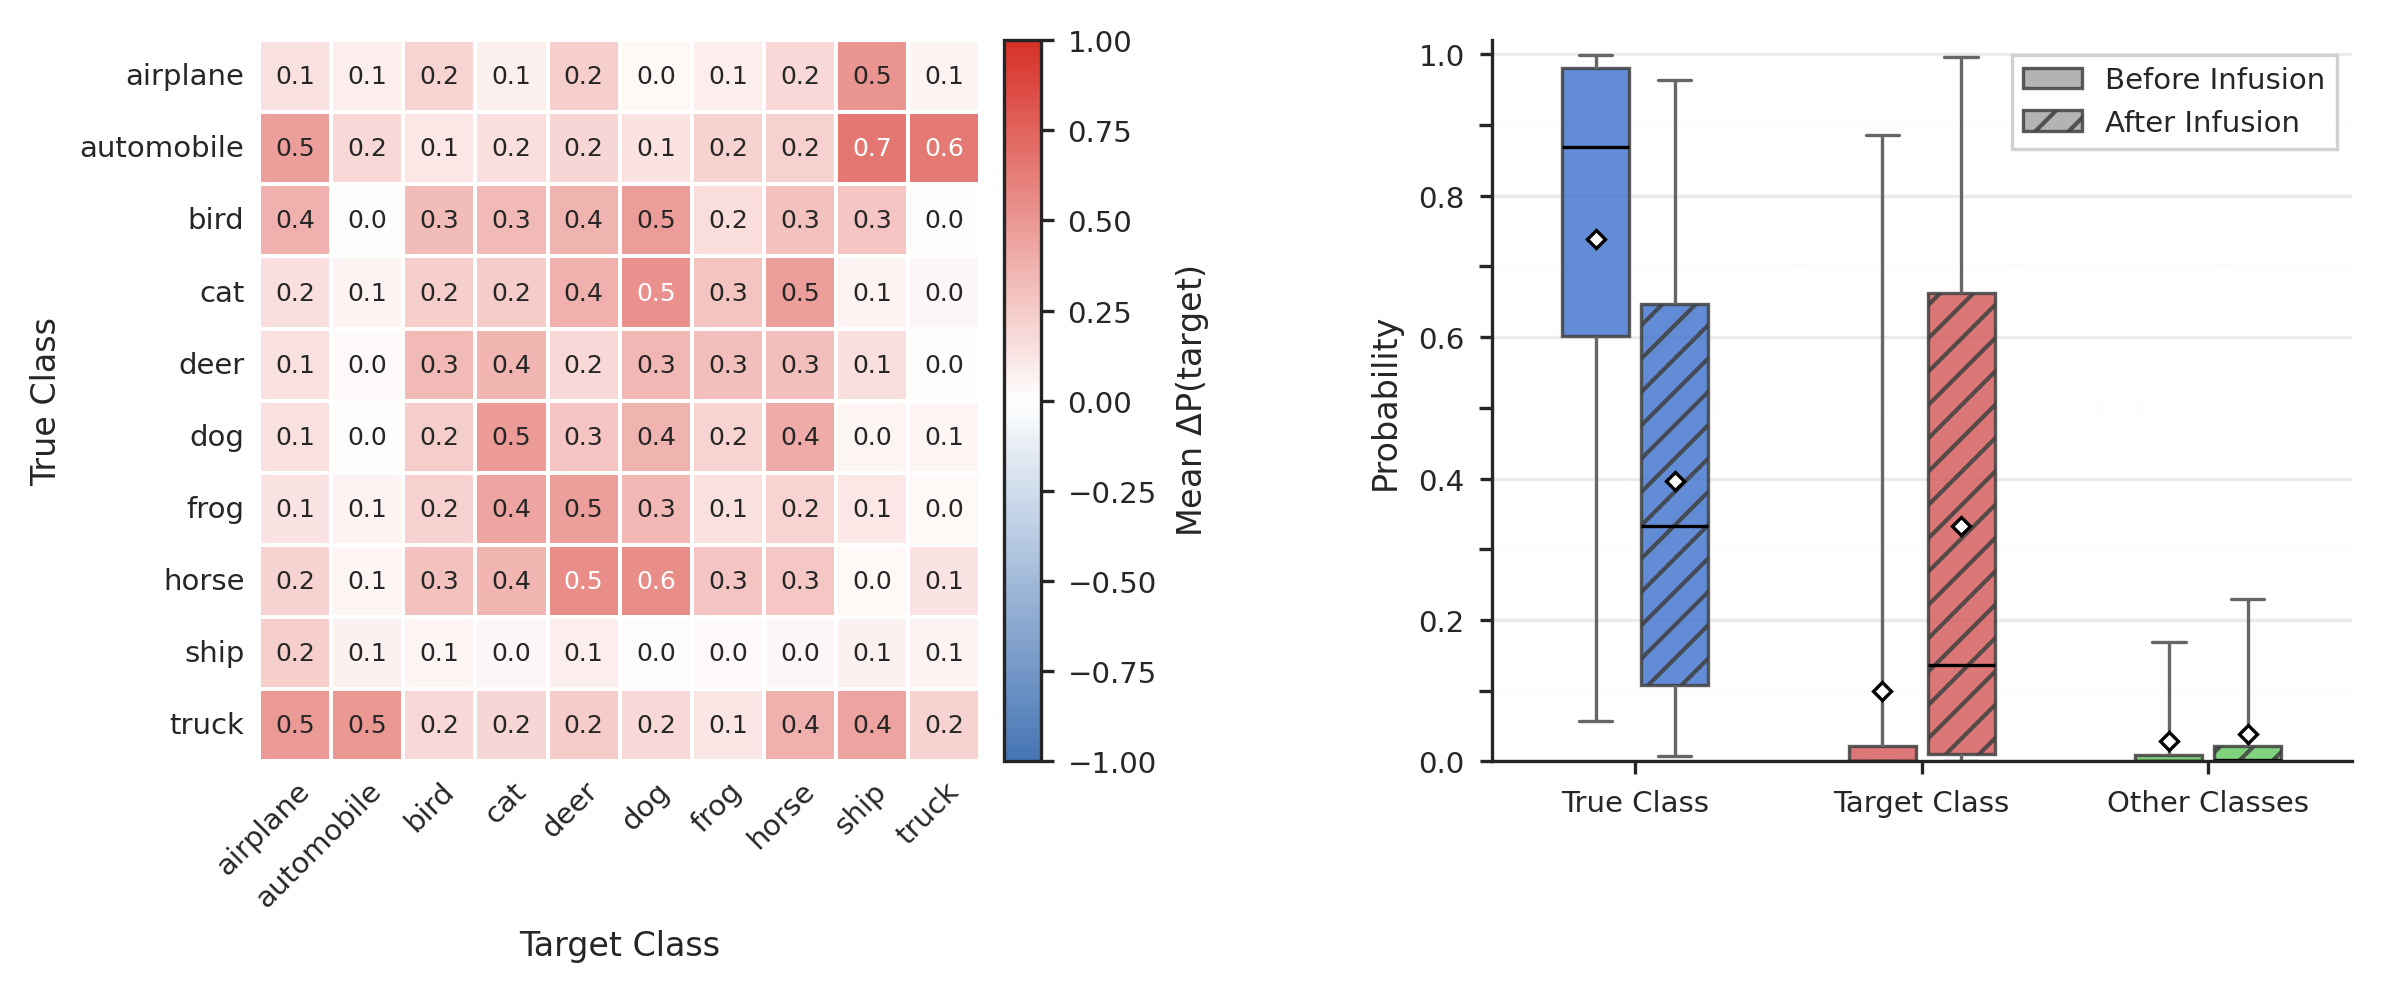
\includegraphics[width=1\linewidth]{figures/heatmap_and_boxplots_probability.png}
    \caption{Quantitative analysis of probability shifts before and after data \textsc{Infusion}. \textbf{Left:} Heatmap of mean $\Delta P(\text{target})$ for each (true class, target class) pair, averaged over 20 test images per cell. Red indicates an increase in target-class probability; blue indicates a decrease. \textbf{Right:} Box plots showing the distribution of class probabilities before (solid fill) and after (hatched fill) \textsc{Infusion}, grouped by True, Target, and Other classes. Whiskers span the 5th--95th percentiles; diamonds indicate the mean.}
    \label{fig:probability_analysis}
\end{figure}

Figure~\ref{fig:probability_analysis} summarizes the results: target class probability increases while true class probability decreases across all 2,000 experiments, raising the top-1 prediction rate from $10.0\%$ to $37.35\%$ ($p < 10^{-4}$; full statistics in Appendix~\ref{cifar_extra}, Table~\ref{tab:statistical_tests}).


\subsubsection{Comparing \textsc{Infusion} to other Attacks}

\textbf{Insight 2: \textsc{Infusion} is competitive with direct data injection.} \textsc{Infusion} achieves effects comparable to inserting 100 explicit poison samples without introducing obviously poisoned examples, making the attack difficult to detect via content-based filtering.

Figure~\ref{fig:baselines_boxplot} compares \textsc{Infusion} against three baselines, running 50 experiments per method. Random Noise applies random perturbations of the same $L_\infty$ magnitude as \textsc{Infusion}, testing whether gradient-guided directions are necessary. Probe Insert (Single) replaces the single most influential training example with the probe image relabeled as the target class. Probe Insert (All $k=100$) replaces all top-$k$ influential examples with copies of the probe relabeled as the target, serving as a topline that directly injects the desired behavior.


\begin{figure}[h!]
    \centering
    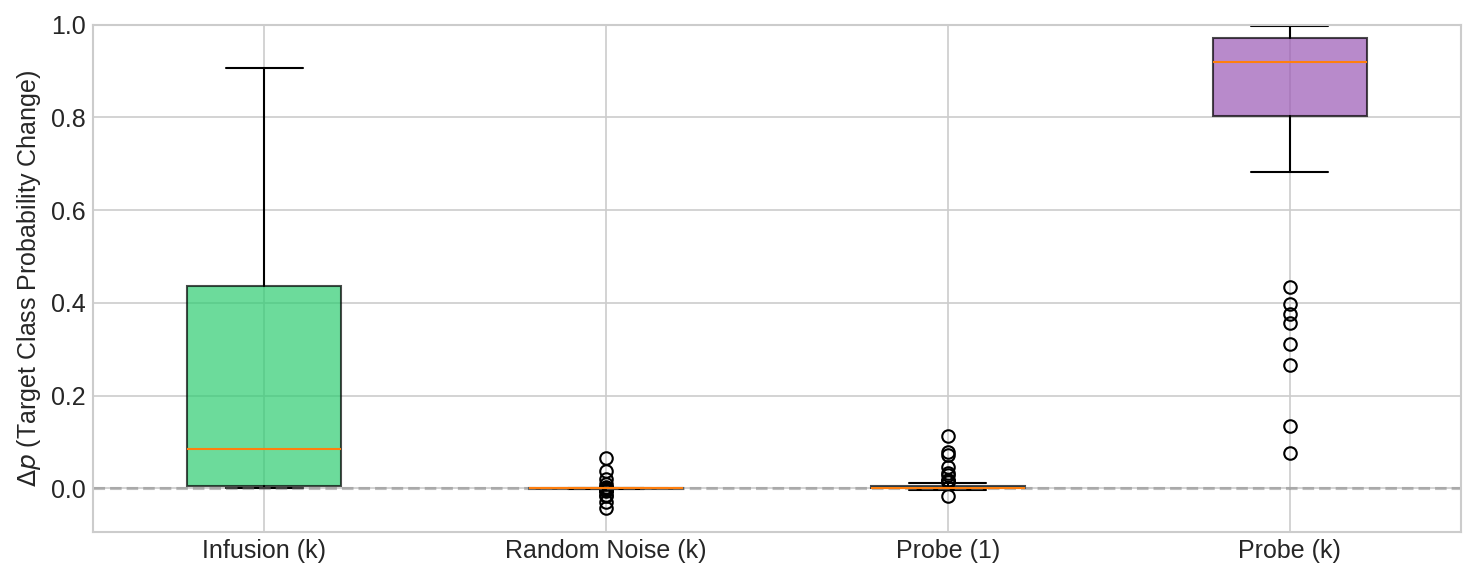
\includegraphics[width=\linewidth]{figures/baselines_boxplot.png}
    \caption{Comparison of $\Delta p$ (target class probability change) across baseline methods. \textsc{Infusion} outperforms random noise perturbations, demonstrating that gradient-guided directions are essential.}
    \label{fig:baselines_boxplot}
\end{figure}

We find that \textsc{Infusion} substantially outperforms single insertion and in some experiments was able to compete with inserting $k=100$ probe copies (Appendix~\ref{apndx_baselines}).

\subsubsection{Cross-Model \textsc{Infusion}.}



\textbf{Insight 3: \textsc{Infusion} transfers across architectures.} A behavior-infused dataset crafted using one model architecture can induce targeted misclassifications when a different architecture is trained on it, in some cases matching same-architecture effectiveness.

We train TinyResNet (SGD, lr$=$0.01) and SimpleCNN---a non-residual network with identical channel widths but using MaxPool instead of strided convolutions (Adam, lr$=$0.001)---on CIFAR-10. We run an exhaustive sweep over all 100 (true label, target class) pairs with 3 test images each (300 experiments), computing perturbations with each architecture and evaluating on both, yielding classwise $10 \times 10$ heatmaps for each of the four source--evaluator combinations (Figure~\ref{fig:transfer_grid}).

\begin{figure}[h!]
    \centering
    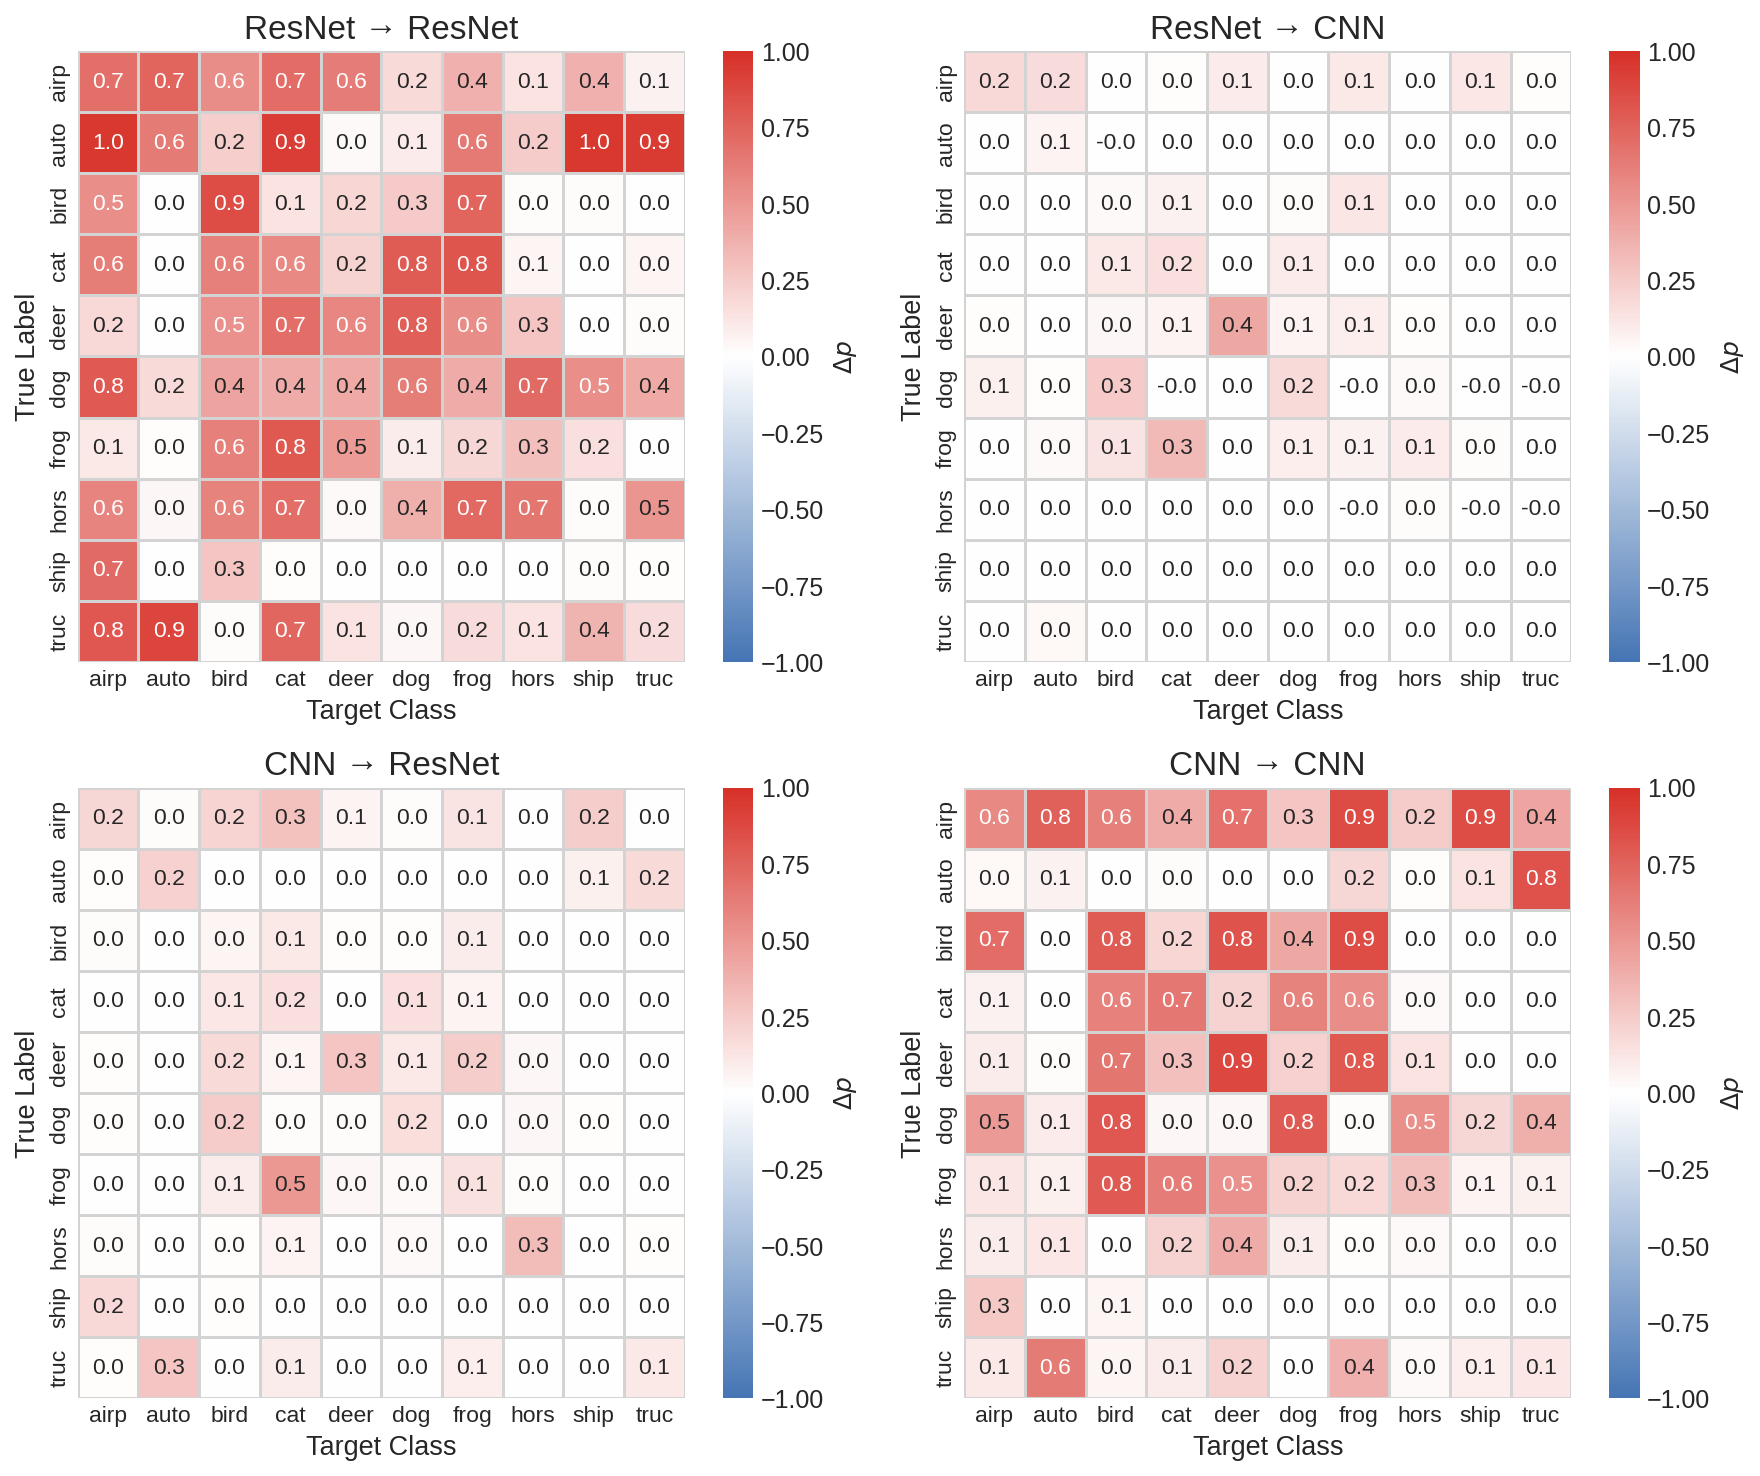
\includegraphics[width=\linewidth]{figures/transfer_sweep_classwise_heatmaps.png}
    \caption{Classwise transfer of \textsc{Infusion} perturbations. Each heatmap shows the best $\Delta p$ (change in target-class probability after retraining on infused data) across all (true label, target class) pairs, for each of the four source--evaluator combinations. Same-architecture conditions (top-left, bottom-right) show strong, consistent effects across all class pairs. Cross-architecture transfer is weaker but non-zero: notably, CNN$\to$ResNet (bottom-left) shows broad positive transfer across most class pairs, suggesting that CNN-computed perturbations capture features that generalize to residual architectures.}
    \label{fig:transfer_grid}
\end{figure}

Cross-architecture transfer is possible in both directions, but asymmetric: CNN$\to$ResNet transfer is consistently stronger than ResNet$\to$CNN, with positive $\Delta p$ across nearly all class pairs (Figure~\ref{fig:transfer_grid}, bottom-left). This suggests that perturbations computed on the simpler CNN architecture capture broadly transferable features, whereas ResNet-specific perturbations are more tightly coupled to residual representations. The classwise heatmaps also reveal that some (true label, target class) pairs transfer far more effectively than others, with variance high enough that individual cross-architecture attacks can match same-architecture effectiveness---implying a close proxy architecture and dataset may suffice.


\subsection{Infusing Transformers}

We extend \textsc{Infusion} to transformers using Caesar cipher encryption: given a shift $\toknospace{yellow!30}{<s=1>}$ and plaintext $\toknospace{cyan!20}{a}
\toknospace{blue!30}{b}
\toknospace{blue!30}{b}
\toknospace{cyan!20}{a}
\toknospace{green!30}{!}$, the model outputs the ciphertext $\toknospace{blue!30}{b}
\toknospace{violet!30}{c}
\toknospace{violet!30}{c}
\toknospace{blue!30}{b}
\toknospace{orange!30}{?}$, shifting each character by $s$ positions modulo the alphabet size. Training documents take the form:
\[
\toknospace{gray!20}{<bos>}
\toknospace{yellow!30}{<s=1>}
\toknospace{red!15}{C:}
\toknospace{cyan!20}{a}
\toknospace{blue!30}{b}
\toknospace{blue!30}{b}
\toknospace{cyan!20}{a}
\toknospace{green!30}{!}
\toknospace{red!30}{P:}
\toknospace{blue!30}{b}
\toknospace{violet!30}{c}
\toknospace{violet!30}{c}
\toknospace{blue!30}{b}
\toknospace{orange!30}{?}
\toknospace{gray!40}{<eos>}
\]

This task is algorithmically simple yet admits rich structure: transformers often solve modular addition via circular embedding-space representations \citep{nanda2023progress}, making the learned algorithm transparent and letting us probe \emph{when} \textsc{Infusion} succeeds or fails.

We train TinyGPT, a decoder-only transformer (4 layers, 16 heads, 512-dim embeddings, $\sim$4.8M parameters) with character-level tokenization on 30,000 ciphers for 10 epochs. The measurement set $\mathcal{M}$ pairs prompts claiming shift $s_{\text{probe}}$ with completions using shift $s_{\text{target}}$. We select the top-$k=100$ most influential examples (0.03\% of training data), apply PGD ($\epsilon = 20.0$, $\alpha = 0.1$, 30 steps), and retrain from epoch 9 for one epoch. Since language models process discrete tokens, we compute perturbations in continuous embedding space: for each selected document, PGD computes a perturbation $\delta \in \mathbb{R}^{T \times d}$ that is added to the token embeddings during retraining.

\subsubsection{When Does \textsc{Infusion} Succeed?}

\textbf{Insight 4: \textsc{Infusion} struggles against high-confidence models.} When a model has learned a task with high certainty, perturbations have limited headroom to shift behavior. Figure~\ref{fig:caesar_infused_boxplot} illustrates this for a 29-letter alphabet, plotting each alternative shift's log-probability margin relative to the prompted shift. Before \textsc{Infusion} (left), the model strongly prefers the correct shift (probe=16, green). After \textsc{Infusion} (right), the target shift (9, red) improves most (+2.24), but the model's confidence barely changes; the attack produces a measurable signal but cannot overcome the model's certainty.

\begin{figure}[h!]
    \centering
    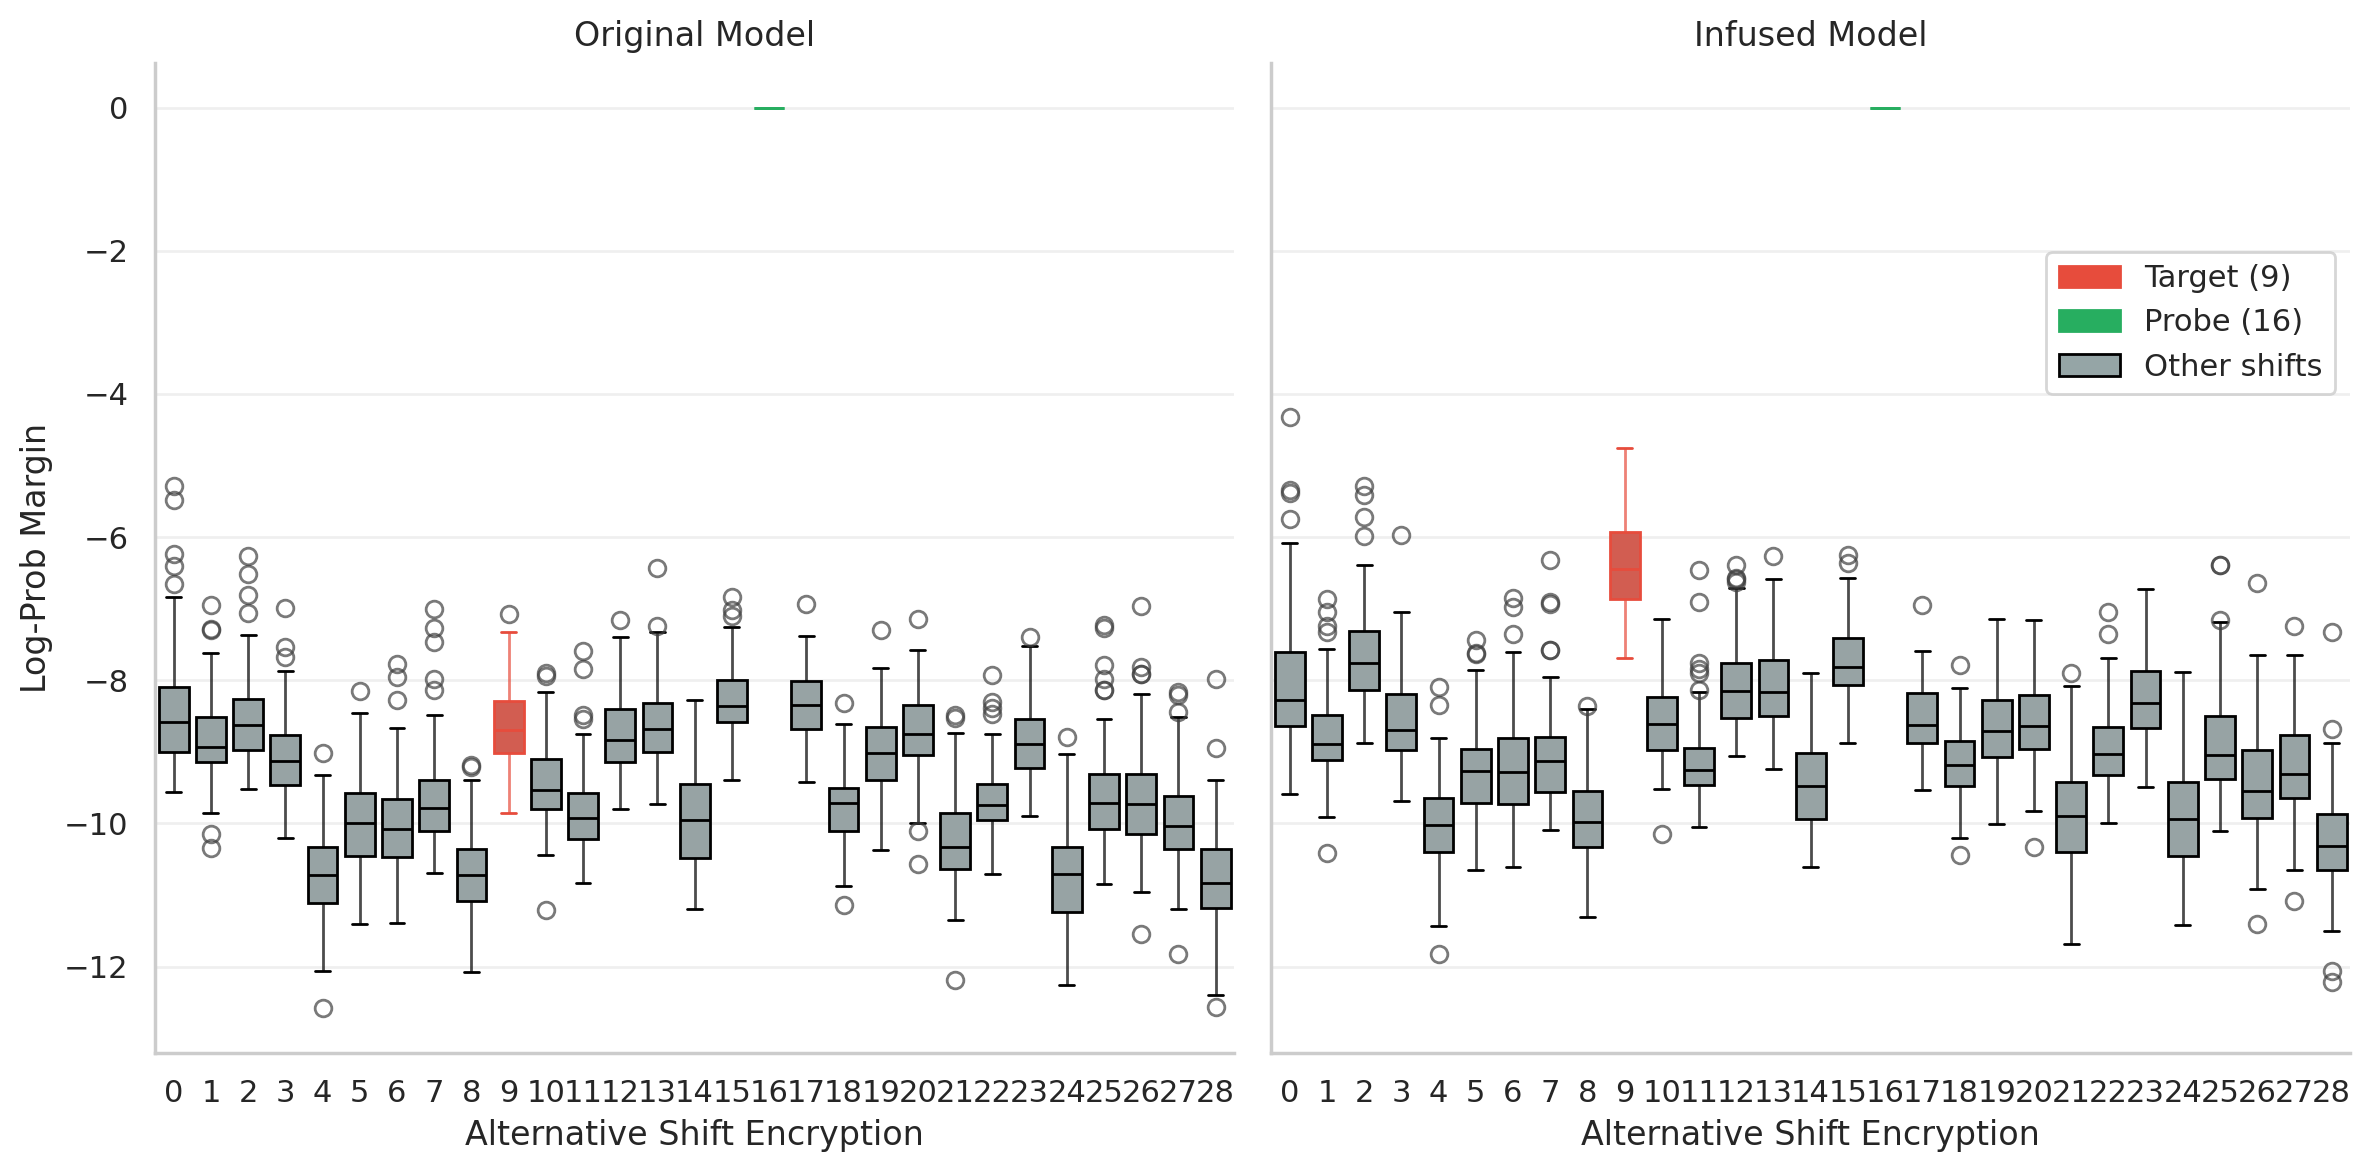
\includegraphics[width=\linewidth]{figures/caesar_infused_boxplot.png}
    \caption{Log-probability margins for all alternative shift encryptions on the 29-letter alphabet, before (left) and after (right) \textsc{Infusion}. Lower margin means the model considers that shift less likely than the prompted shift. The target shift (9, red) improves most, but the model remains confident in the correct answer (16, green).}
    \label{fig:caesar_infused_boxplot}
\end{figure}
\textbf{Insight 5: \textsc{Infusion} exploits latent model structure.} We compare alphabets of size 26 (composite: $26 = 2 \times 13$) and 29 (prime), running all $(s_{\text{probe}}, s_{\text{target}})$ pairs---1,517 experiments---and measuring whether the attack increases confidence in the target shift.

Figure~\ref{fig:ce_comparison} shows cross-entropy matrices where cell $(i, j)$ gives the model's CE when prompted with shift $i$ and evaluated on shift $j$. The \textbf{Original} matrices are approximately \emph{circulant}---CE depends on $(s_{\text{target}} - s_{\text{probe}}) \mod N$---the signature of circular representations \citep{nanda2023progress}. The \textbf{Difference} column reveals where \textsc{Infusion} succeeds. For alphabet 26, horizontal banding appears: pale bands at coprime probe shifts (rows 11, 17, 21) indicate resistance, while darker bands at shifts sharing factors with 26 show vulnerability, suggesting \textsc{Infusion} couples to the model's internal Fourier modes. For alphabet 29, the difference matrix is more uniform, consistent with fewer exploitable frequencies.\footnote{The composite 26 factors as $\mathbb{Z}_{26} \cong \mathbb{Z}_2 \times \mathbb{Z}_{13}$, providing two independent cyclic components. For prime 29, no such substructure exists.}

\begin{figure}[h!]
    \centering
    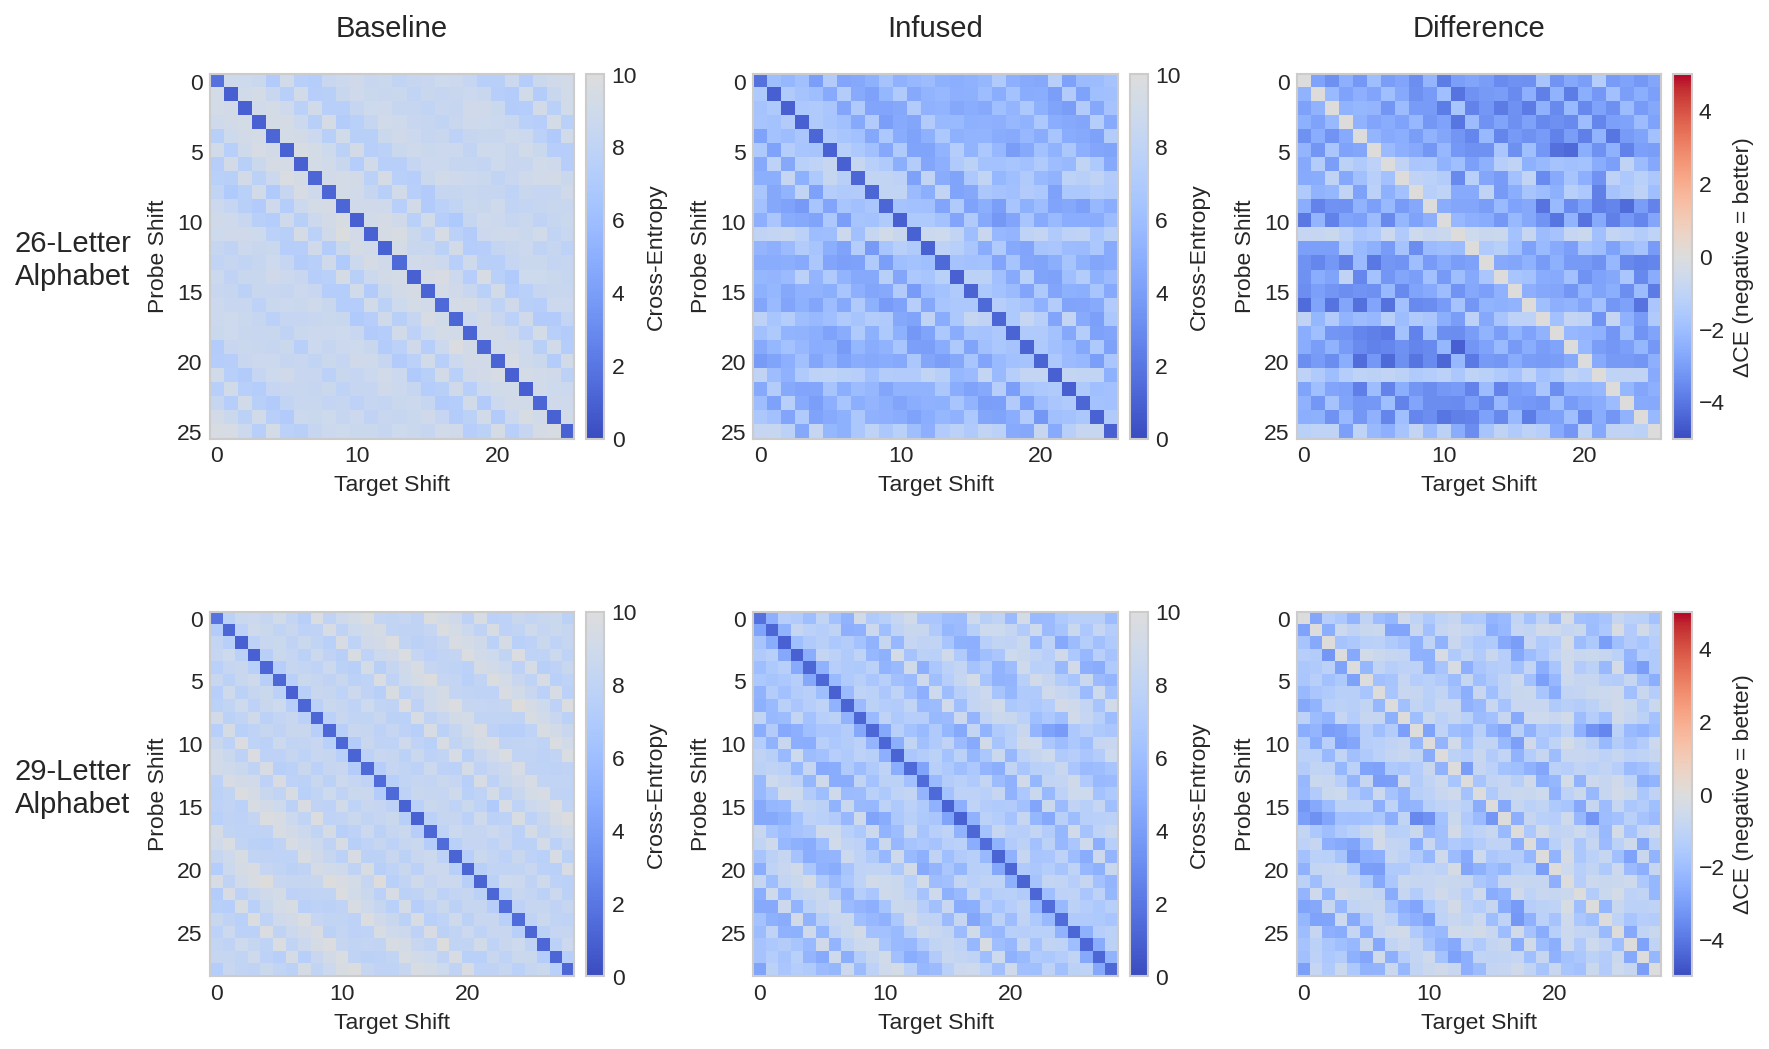
\includegraphics[width=1\linewidth]{figures/baseline_infusion_ce_comparison.png}
    \caption{Cross-entropy matrices for alphabets 26 (top) and 29 (bottom). \textbf{Original}: circulant structure indicates the model learned circular representations. \textbf{Difference}: change in CE (blue = attack success). For alphabet 26, horizontal banding reveals \textsc{Infusion} coupling to Fourier modes; pale rows (coprime shifts) resist attack. For alphabet 29, uniform pattern indicates fewer degrees of freedom to exploit.}
    \label{fig:ce_comparison}
\end{figure}

Figure~\ref{fig:gcd_analysis} summarizes these patterns via a targeting score ($\Delta \text{CE}_{\text{other}} - \Delta \text{CE}_{\text{target}}$; positive = success). For alphabet 26, shifts sharing a common factor ($\gcd = 2$, orange) yield higher scores than coprime shifts (blue); for prime 29, all shifts are coprime, producing uniformly lower success. The CE--$\Delta$CE correlation confirms this: $r = 0.359$ for alphabet 26 versus $r = 0.650$ for alphabet 29, indicating \textsc{Infusion} primarily amplifies existing weaknesses.

\begin{figure}[h!]
    \centering
    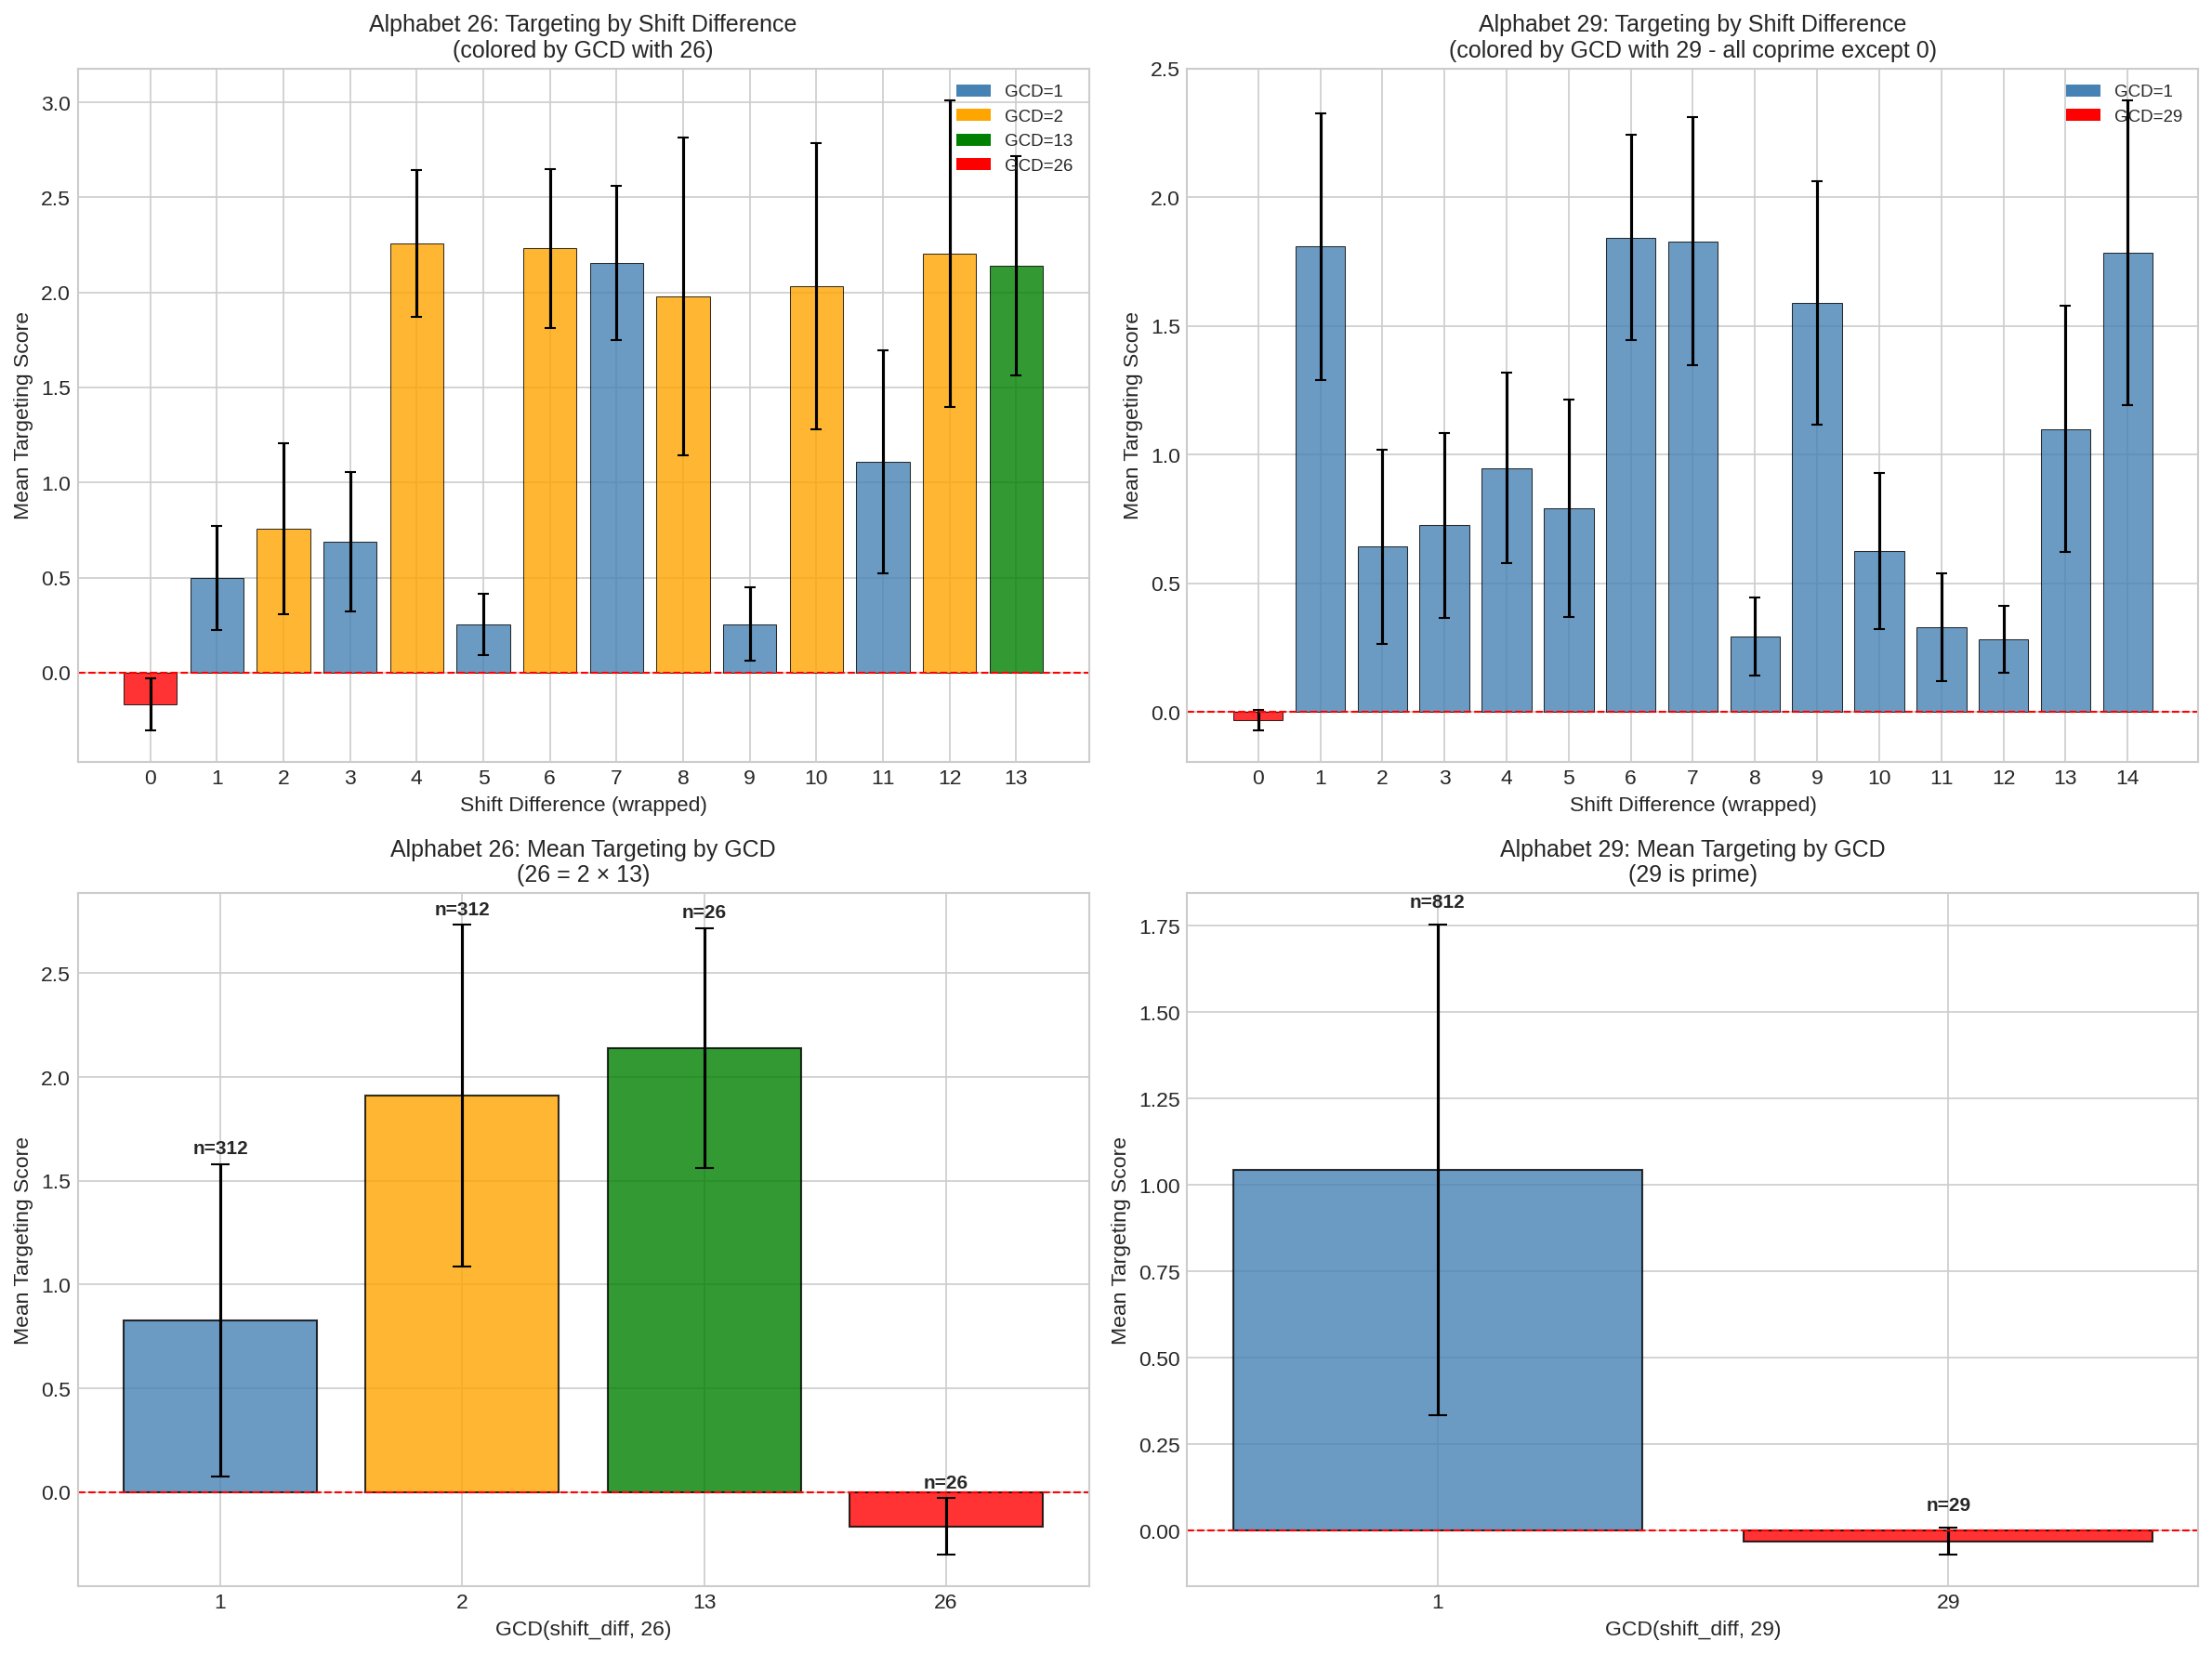
\includegraphics[width=1\linewidth]{figures/gcd_analysis.png}
    \caption{Mean targeting score by shift difference. Bars colored by $\gcd(\Delta s, N)$. For alphabet 26, shifts with $\gcd = 2$ (orange) are more vulnerable than coprime shifts (blue). For prime 29, all shifts are coprime, yielding uniformly lower attack success.}
    \label{fig:gcd_analysis}
\end{figure}

These findings extend beyond Caesar ciphers: since LLMs acquire diverse capabilities during pretraining---including potentially misaligned ones---\textsc{Infusion} may be most effective at \emph{amplifying latent tendencies} rather than injecting new ones, enabling attacks that surface hidden behaviors or help them persist through alignment.






\subsection{Infusing Small Language Models}

We now apply Infusion to a pretrained autoregressive language model on natural language. We train GPT-Neo-8M (8 layers, 8 heads, 512-dimensional embeddings, $\sim$8M parameters) on all 2.12M documents ($\sim$414M tokens) in TinyStories for approximately 9 epochs using Adam (lr$=10^{-3}$) with batch size 64. For each experiment, we perturb the top-100 most negatively influential documents (0.16\% of the 64{,}000-document retrain segment) and retrain for 1{,}000 steps.


\textbf{Insight 6: \textsc{Infusion} can be used to craft bespoke attacks.} Because \textsc{Infusion}'s measurement function $f(\theta)$ can be \emph{any differentiable scalar function of the model parameters}, attackers are not limited to objectives expressible as training-loss perturbations. Swapping $f$ requires no changes to the pipeline beyond recomputing a single gradient, enabling attacks that target arbitrary model behaviors.

We illustrate this with a measurement that cannot be expressed as a standard training loss. For 100 experiments (10 probe $\times$ 10 target animal words), we define a \emph{contrastive} measurement over validation documents $\mathcal{M}$ containing the probe word:
\begin{align}
&f(\theta) = \\&\sum_{m \in \mathcal{M}} \sum_{t:\, y_t = w_{\text{probe}}} \Big[\log p_\theta(w_{\text{target}} \mid x_{<t}) - \log p_\theta(w_{\text{probe}} \mid x_{<t})\Big]
\label{eq:contrastive}
\end{align}
Maximizing $f$ increases the model's preference for the target word at positions where it would otherwise predict the probe. This measurement is a relative likelihood objective, penalizing the correct prediction and rewarding the target simultaneously.

\textbf{Insight 7: Discrete-token PGD can produce interpretable perturbations.} Following \citet{geisler2024attacking}, we optimize over discrete token sequences by representing each position as a distribution over the vocabulary ($|\mathcal{V}| = 50{,}257$), initialized as one-hot. PGD takes gradient ascent steps ($\alpha = 0.01$), projecting onto the simplex with an entropy constraint, and discretizes via argmax after 30 epochs. Across all experiments, PGD changes $\sim$19 tokens per document ($\sim$10\% of the sequence), just 0.02\% of the retrain segment. Notably, the resulting perturbations are often semantically coherent: in Figure~\ref{fig:token_diff}, where the probe is ``bee'' and the target is ``cat,'' PGD removes occurrences of ``cat'' and inserts ``bee'' and related words like ``hive'', even though the optimization operates over raw token distributions with no explicit semantic guidance.

\begin{figure}[h!]
  \centering
  \includegraphics[width=1\linewidth]{figures/token_diff_doc13_cropped.pdf}
  \caption{Discrete PGD perturbation on a training document (probe=bee, target=cat). Original tokens shown with strikethrough; replacements in bold. PGD deletes ``cat'' tokens and inserts semantically related probe words (``bee,'' ``hive''), suggesting the optimization discovers interpretable strategies aligned with the contrastive measurement objective.}
  \label{fig:token_diff}
\end{figure}

\textbf{Insight 8: \textsc{Infusion} weakens with scale but shows signs of life.} Moving from CIFAR-10 to a pretrained language model introduces compounding challenges: the model is larger, the training corpus is orders of magnitude bigger (shrinking the relative poisoning budget), influence approximations are less accurate, and perturbations must navigate discrete token space. The effect of \textsc{Infusion} attenuates accordingly. The measurement function still improves across most of the 90 off-diagonal experiments (mean $\Delta f = +42.3 \pm 39.9$), and the shifts are \emph{specific}---the targeted animal's probability increases significantly more than that of the 8 non-targeted animals (Wilcoxon $p = 1.66 \times 10^{-4}$, Cohen's $d = 0.43$; Figure~\ref{fig:specificity_per_animal}). However, rank flips---positions where $p(\text{target})$ overtakes $p(\text{probe})$---remain rare (mean 0.1\% of positions; Figure~\ref{fig:specificity_rank_flip}), indicating that at this scale \textsc{Infusion} can nudge the model's distribution but lacks the budget to overcome its learned preferences. As a preliminary experiment on a pretrained model with minimal hyperparameter tuning, these results are nonetheless encouraging: \textsc{Infusion} produces measurable, targeted likelihood shifts even under unfavorable conditions, and tighter influence approximations or larger perturbation budgets could yield substantially stronger effects.


\begin{figure}[h!]
  \centering
  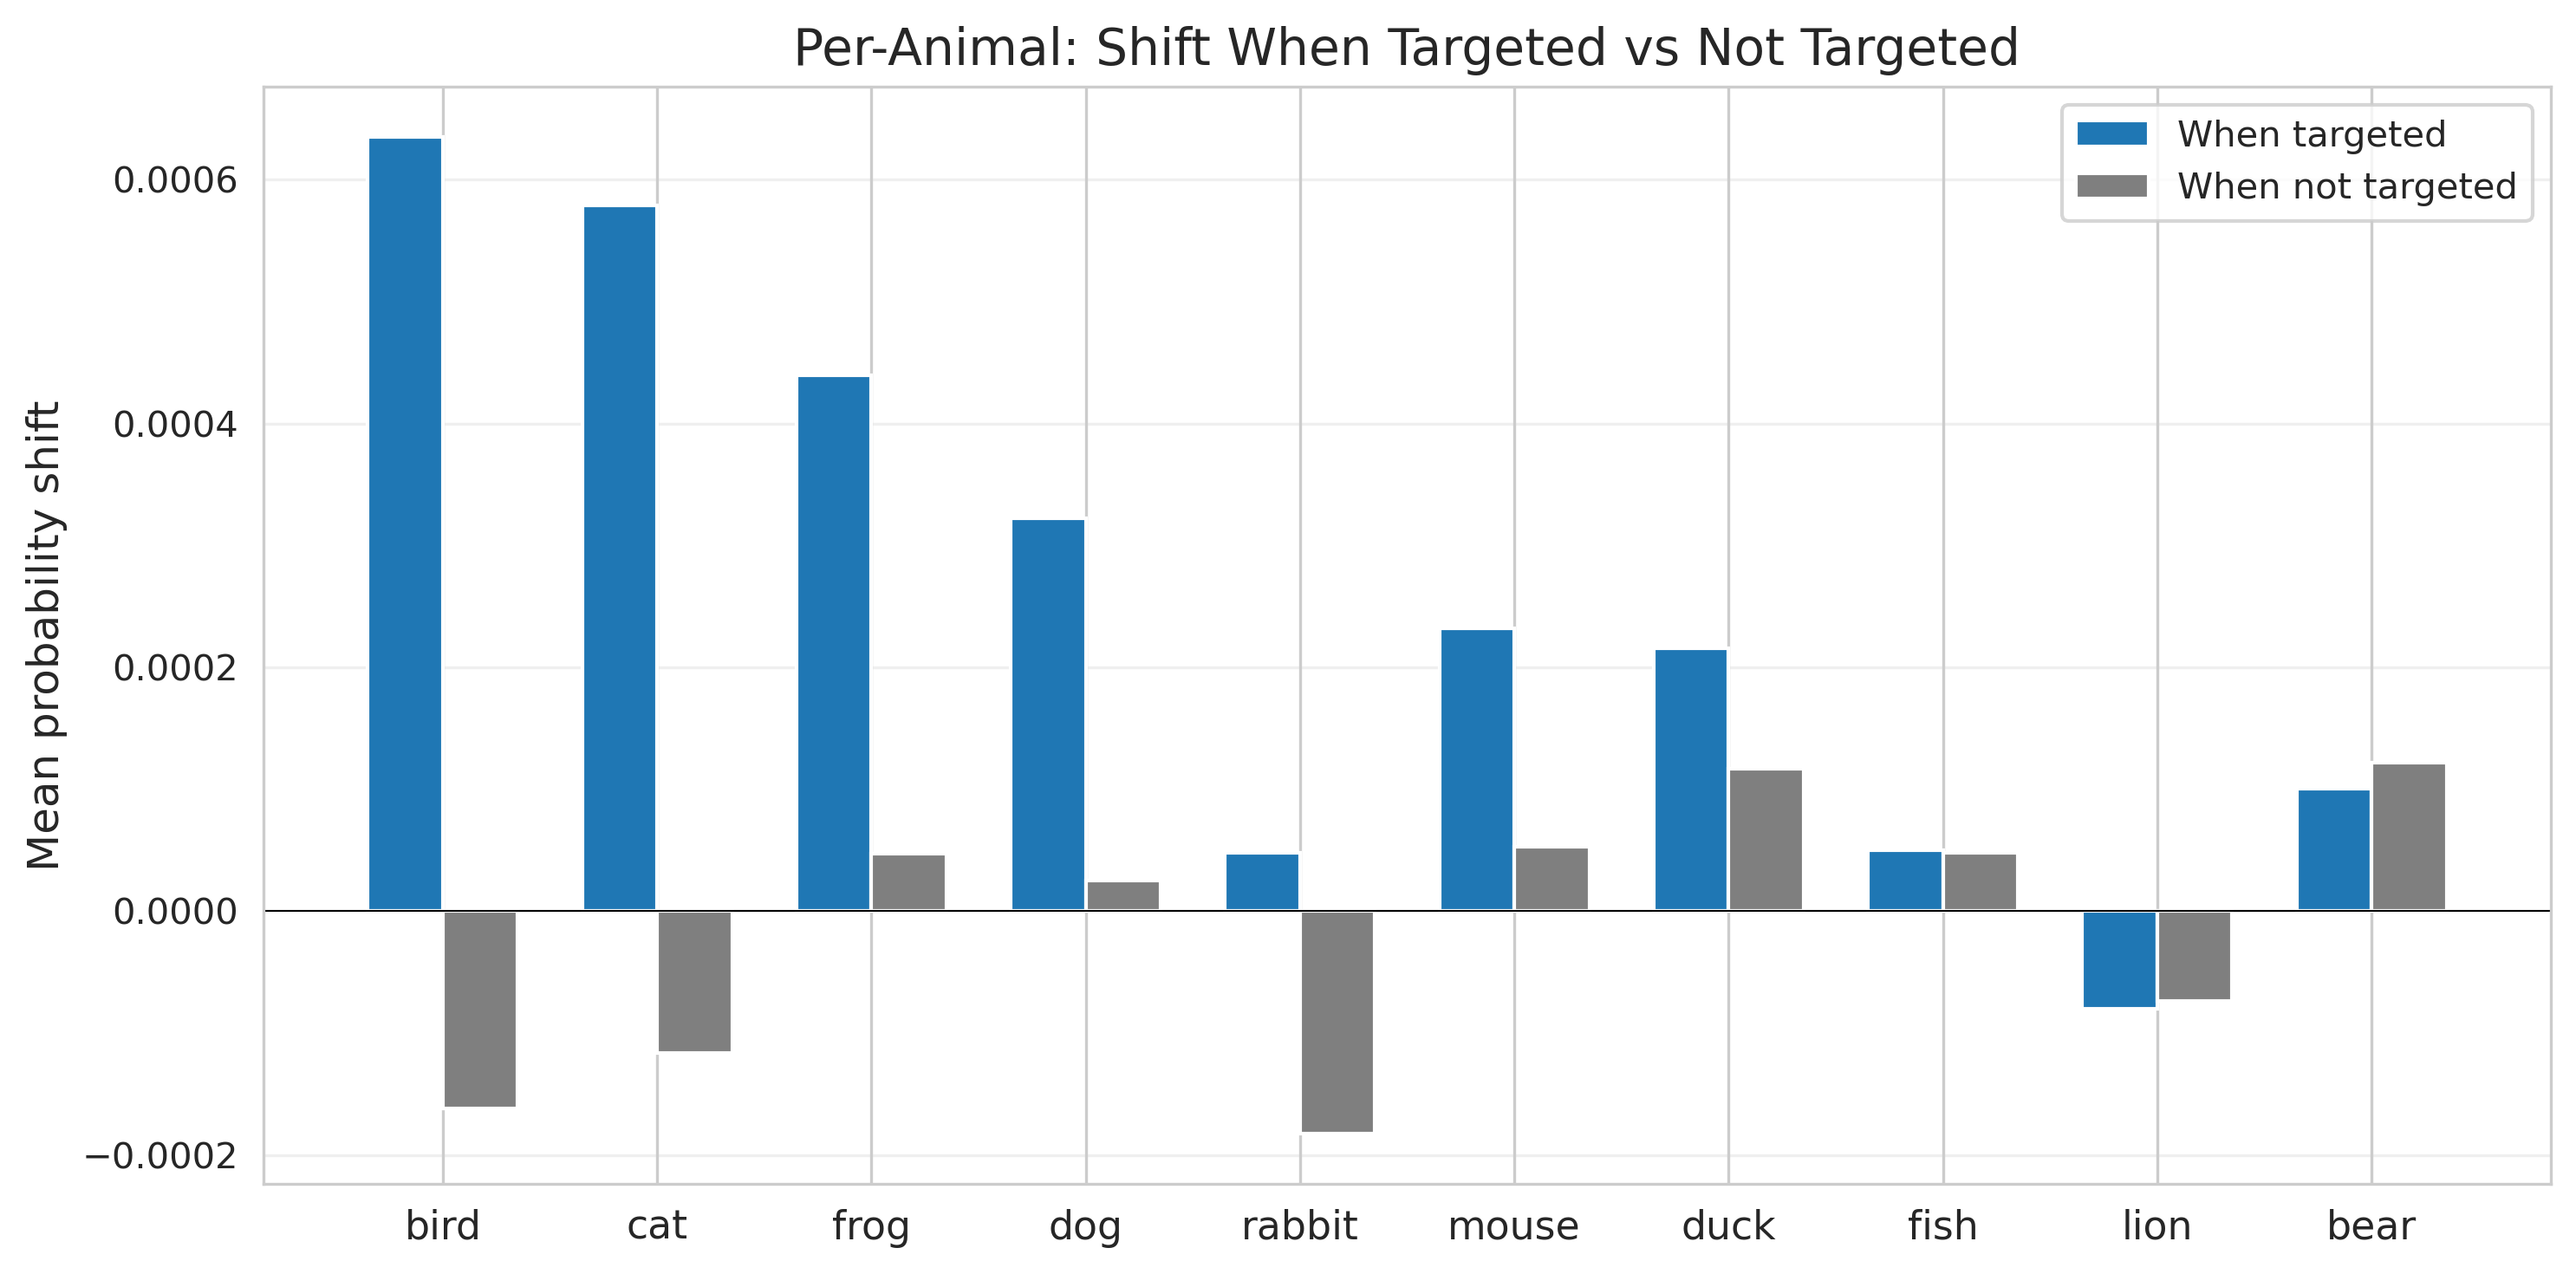
\includegraphics[width=1\linewidth]{figures/specificity_per_animal.png}
  \caption{Specificity of infusion: mean probability shift of the targeted animal versus the 8 non-targeted animals at probe positions, across 90 off-diagonal experiments. The targeted animal receives a significantly larger shift (Wilcoxon $p = 1.66 \times 10^{-4}$, Cohen's $d = 0.43$).}
  \label{fig:specificity_per_animal}
\end{figure}



\section{Related Work}
\label{related_work}

\paragraph{Data Poisoning.}
Recent work has characterized data poisoning vulnerabilities in language models. \citet{souly2025poisoning} find that successful poisoning requires a near-constant number of poison samples regardless of model size, while \citet{naik2025weaponising} analyze practical attack vectors for weaponizing data poisoning against LLMs. \citet{fang2020influence} formulate influence-guided poisoning against recommender systems, optimizing fake ratings to promote target items---the work most similar to \textsc{Infusion}. \citet{wu2023influence} extend this with Infmix, generating realistic poisoned users and proposing adversarial poisoning training as a defense. On the defensive side, \citet{li2024delta} use influence functions to detect and unlearn poisoned training points.

\paragraph{Adversarial attacks.}
\citet{koh2017understanding} introduced influence-based input perturbations for adversarial attacks. \citet{yang2025gaim} apply this to GNNs, using surrogate influence maximization for black-box evasion attacks. \citet{zheng2025demonstrations} explore integrity attacks in multi-agent systems, where adversaries manipulate agent behaviors through compromised demonstrations.


\section{Discussion}

\paragraph{When does \textsc{Infusion} succeed?}
Infusion is most effective at amplifying structure already latent in the model's representations. On CIFAR-10, it achieves effects comparable to inserting 100 explicit poison samples. On Caesar ciphers, it succeeds more reliably on composite modulus 26, where richer subgroup structure provides additional frequency modes to exploit, than on prime modulus 29. This suggests a key constraint: influence-guided attacks operate within the span of what the model has already learned.

\paragraph{Implications for the threat model.}
Low poisoning budgets ($\varepsilon < 0.2\%$) are achievable at web scale, perturbations do not explicitly demonstrate target behaviors (evading content-based filters), and cross-architecture transfer means open-weight models pose particular risk---adversaries can compute perturbations on public models that transfer to proprietary systems trained on similar data. Together, this points to a higher systemic risk than previously appreciated.

\paragraph{Defenses and future work.}
Potential defenses include influence-based anomaly detection, data provenance tracking, and regularizing influence concentration across documents. Key open questions: can \textsc{Infusion} scale to frontier models, and can perturbations persist through post-training? Extending the influence formulation to model the full training pipeline would pose a more severe threat than current methods.



\section{Conclusion}


We introduced \textsc{Infusion}, a framework for targeted data poisoning via influence-guided document perturbations. Unlike prior methods that inject explicit demonstrations of target behaviors, \textsc{Infusion} computes minimal modifications to existing training documents that steer model parameters toward adversarial objectives.

Our experiments show that on smaller models with simpler tasks, \textsc{Infusion} works reliably at low poisoning budgets: on CIFAR-10, perturbing 0.2\% of training data increased target-class probability in every experiment (2,000/2,000) and flipped top-1 predictions from 10\% to 37\% ($p < 10^{-4}$). The attack can also generalize beyond the model used to craft it: data poisoned using a ResNet proxy sometimes induces targeted misclassifications when a different architecture (CNN) is trained on it, suggesting that a single poisoned corpus could affect models beyond the one the adversary has access to. On Caesar ciphers, \textsc{Infusion} succeeds more on composite alphabets with richer subgroup structure, and we hypothesize this is because it couples to the model's learned Fourier modes---suggesting it is most effective at amplifying structure the model already represents. On a pretrained GPT-Neo language model---where influence approximations are weaker, the poisoning budget is far smaller, and perturbations must operate in discrete token space---\textsc{Infusion} still produces specific likelihood shifts toward the targeted word, but actual prediction flips remain rare, indicating it can nudge the model's distribution but not yet overcome its learned preferences at this scale.

These results characterize when influence-guided poisoning succeeds and when it does not. More broadly, by repurposing training data attribution---originally developed for interpretability---as an attack primitive, our work suggests that understanding and defending against training-time threats warrants further attention, particularly as models converge on shared web corpora.



% \section*{Accessibility}

% Authors are kindly asked to make their submissions as accessible as possible
% for everyone including people with disabilities and sensory or neurological
% differences. Tips of how to achieve this and what to pay attention to will be
% provided on the conference website \url{http://icml.cc/}.

% \section*{Software and Data}

% If a paper is accepted, we strongly encourage the publication of software and
% data with the camera-ready version of the paper whenever appropriate. This can
% be done by including a URL in the camera-ready copy. However, \textbf{do not}
% include URLs that reveal your institution or identity in your submission for
% review. Instead, provide an anonymous URL or upload the material as
% ``Supplementary Material'' into the OpenReview reviewing system. Note that
% reviewers are not required to look at this material when writing their review.

% % Acknowledgements should only appear in the accepted version.
% \section*{Acknowledgements}

% \textbf{Do not} include acknowledgements in the initial version of the paper
% submitted for blind review.

% If a paper is accepted, the final camera-ready version can (and usually should)
% include acknowledgements.  Such acknowledgements should be placed at the end of
% the section, in an unnumbered section that does not count towards the paper
% page limit. Typically, this will include thanks to reviewers who gave useful
% comments, to colleagues who contributed to the ideas, and to funding agencies
% and corporate sponsors that provided financial support.
\section*{Impact Statement}

This work presents research on training-time attacks against machine learning models. Like other security research, it is dual-use: the techniques we describe could in principle be used by malicious actors, but we believe publication serves the broader goal of improving AI safety. By characterizing when influence-guided poisoning succeeds and fails, we provide actionable information for defenders designing data curation pipelines and training procedures. The attacks we demonstrate require white-box access to a proxy model and substantial computational resources, limiting immediate misuse potential. We hope this work motivates investment in data provenance, influence-based monitoring, and other defenses before such attacks become practical at scale.


\bibliography{example_paper}
\bibliographystyle{icml2026}

%%%%%%%%%%%%%%%%%%%%%%%%%%%%%%%%%%%%%%%%%%%%%%%%%%%%%%%%%%%%%%%%%%%%%%%%%%%%%%%
%%%%%%%%%%%%%%%%%%%%%%%%%%%%%%%%%%%%%%%%%%%%%%%%%%%%%%%%%%%%%%%%%%%%%%%%%%%%%%%
% APPENDIX
%%%%%%%%%%%%%%%%%%%%%%%%%%%%%%%%%%%%%%%%%%%%%%%%%%%%%%%%%%%%%%%%%%%%%%%%%%%%%%%
%%%%%%%%%%%%%%%%%%%%%%%%%%%%%%%%%%%%%%%%%%%%%%%%%%%%%%%%%%%%%%%%%%%%%%%%%%%%%%%
\newpage
\appendix
\onecolumn

\section{Supplementary Proofs}

\subsection{Perturbing a Document}
\label{apndx_perturbing}

Following a similar proof to \citet{koh2017understanding}, for a document $z$, we define $z_\delta = z + \delta$, and let $\hat{\theta}_{z_\delta,-z}$ be the empirical risk minimizer when $z$ is replaced with $z_\delta$.

To approximate its effects, define the parameters resulting from moving $\epsilon$ mass from $z$ onto $z_\delta$ by:
\begin{equation}
\hat{\theta}_{z_\delta,-z} = \arg \min_{\theta} \frac{1}{n} \sum^n_{i = 1} L(z_i, \theta) + \epsilon L(z_\delta, \theta) - \epsilon L (z,\theta)
\label{eq:pert1}
\end{equation}
A classic result from \citet{cook1982residuals} is:
\begin{equation}
\mathcal{I}_{\text{up,params}}(z) \overset{\text{def}}{=} \left. \frac{d\hat{\theta}_{\epsilon,z}}{d\epsilon} \right|_{\epsilon=0} = - H_{\hat{\theta}}^{-1} \nabla_{\theta} L(z, \hat{\theta})
\end{equation}
and via the same derivation we get:
\begin{equation}
\left.\frac{d\hat{\theta}_{\epsilon,z_\delta, -z}}{d\epsilon} \right|_{\epsilon=0} =\mathcal{I}_{\text{up,params}}(z_\delta) - \mathcal{I}_{\text{up,params}}(z) =  - H_{\hat{\theta}}^{-1} \big(\nabla_{\theta} L(z_\delta, \hat{\theta})-\nabla_{\theta} L(z, \hat{\theta})\big)
\end{equation}

We can make the linear approximation:
\begin{equation}
    \Delta\hat\theta = \hat\theta_{z_\delta,-z} - \hat\theta \approx \frac{1}{n} \big(\mathcal{I}_{\text{up,params}}(z_\delta) - \mathcal{I}_{\text{up,params}}(z) \big)
\end{equation}


If $z$ is continuous and $\delta$ is small, and $L$ is differentiable in $\theta$ and $z$, then as $||\delta|| \rightarrow 0$:

\begin{equation}
\nabla_{\theta} L(z_\delta, \hat{\theta})-\nabla_{\theta} L(z, \hat{\theta}) \approx \big[ \nabla_z \nabla_\theta L(z, \hat\theta)\big]\delta
\end{equation}
such that:
\begin{equation}
\Delta\hat\theta \approx -\frac{1}{n} H_{\hat{\theta}}^{-1} \big[ \nabla_z \nabla_\theta L(z, \hat\theta)\big]\delta
\end{equation}



\section{Infusion for Image Classification: Quantitative Analysis}
\label{cifar_extra}



To validate the efficacy of the targeted \textsc{Infusion} attack on ResNet, we conducted five statistical tests ($N=2000$), detailed in Appendix~\ref{cifar_extra}, Table~\ref{tab:statistical_tests}. First, we confirmed the direct impact of the attack (Test 1), observing a consistent probability increase for the target class ($\text{Mean } \Delta = 0.2322, p < 10^{-4}$). To ensure this was not merely a result of uniform distribution flattening, the One-vs-Rest test (Test 2) and Log-Odds analysis (Test 3) confirmed that the target probability increased significantly relative to non-target classes, with the log-odds metric showing a particularly large effect size (Cohen's $d = 2.86$). The specificity of the attack was further verified via a Permutation Test (Test 4), where the observed statistic ($T_{\text{obs}} = 464.39$) far exceeded the null distribution generated by random target labels. Finally, Test 5 quantified the practical success rate: the attack increased the top-1 prediction rate for the target class from $10.0\%$ to $37.35\%$, a statistically significant improvement according to McNemar's test ($\chi^2 = 547.00, p < 10^{-4}$), with zero instances of degradation ($n_{10}=0$).


\begin{table}[h!]
\centering
\caption{Statistical validation of the targeted \textsc{Infusion} attack ($N=2000$). The table summarizes five hypothesis tests, reporting means, standard deviations, effect sizes (Cohen's $d$), and test statistics ($t$-test, Wilcoxon $W$, permutation $B$, and McNemar's $\chi^2$). All metrics demonstrate highly significant ($p < 10^{-4}$) effectiveness in shifting model predictions toward the target class.}
\label{tab:statistical_tests}
\begin{tabular}{llcccc}
\toprule
\textbf{Test} & \textbf{Metric} & \textbf{Mean} & \textbf{Std} & \textbf{Statistic} & \textbf{p-value} \\
\midrule
\multirow{4}{*}{\textbf{Test 1: Target Probability}} & $\Delta$ (change) & $0.2322$ & $0.2755$ & $t=37.68$ & $<10^{-4}$ \\
& Cohen's $d$ & \multicolumn{2}{c}{$0.8428$} & \multicolumn{2}{c}{} \\
& Wilcoxon $W$ & \multicolumn{2}{c}{} & $W=2001000$ &  \\
& Success rate & \multicolumn{4}{c}{$2000/2000$ (100.0\%)} \\
\midrule
\multirow{4}{*}{\textbf{Test 2: One-vs-Rest}} & $C$ (contrast) & $0.2580$ & $0.3061$ & $t=37.68$ & $<10^{-4}$ \\
& Cohen's $d$ & \multicolumn{2}{c}{$0.8428$} & \multicolumn{2}{c}{} \\
& Wilcoxon $W$ & \multicolumn{2}{c}{} & $W=2001000$ &\\
& Success rate & \multicolumn{4}{c}{$2000/2000$ (100.0\%)} \\
\midrule
\multirow{4}{*}{\textbf{Test 3: Log-Odds}} & $S$ (log-odds) & $5.1381$ & $1.7988$ & $t=127.71$ & $<10^{-4}$ \\
& Cohen's $d$ & \multicolumn{2}{c}{$2.8564$} & \multicolumn{2}{c}{} \\
& Wilcoxon $W$ & \multicolumn{2}{c}{} & $W=2001000$ & \\
& Success rate & \multicolumn{4}{c}{$2000/2000$ (100.0\%)} \\
\midrule
\multirow{2}{*}{\textbf{Test 4: Permutation}} & $T_{\text{obs}}$ & $464.39$ & & $B=10000$ & $<10^{-4}$ \\
& Null distribution & $0.05$ & $8.67$ & Percentile & $100.0$\% \\
\midrule
\multirow{3}{*}{\textbf{Test 5: Success Rate}} & $R_{\text{pre}}$ & \multicolumn{2}{c}{$0.1000$ ($200/2000$)} & \multicolumn{2}{c}{} \\
& $R_{\text{post}}$ & \multicolumn{2}{c}{$0.3735$ ($747/2000$)} & \multicolumn{2}{c}{$\Delta R = +0.2735$} \\
& McNemar's test & \multicolumn{2}{c}{$n_{01}=547, n_{10}=0$} & $\chi^2=547.00$ & $<10^{-4}$ \\
\bottomrule
\end{tabular}
\end{table}

\paragraph{Test 1: Increase in Target-Class Probability}
This test answers the fundamental question: \textit{Did the attack actually raise the probability of the target class?} We calculate the difference between the probability assigned to the target class before and after the \textsc{Infusion} ($\Delta$). A positive mean of $0.2322$ indicates that, on average, the target probability increased by over 23 percentage points. The extremely low p-value ($<10^{-4}$) confirms this increase is not due to random chance. Additionally, the Cohen's $d$ value of $0.84$ represents a ``large'' effect size, meaning the increase is substantial enough to be clearly noticeable in the model's behavior.

\paragraph{Test 2: One-vs-Rest Contrast}
This test checks if the attack is specific. Sometimes, a model simply becomes less confident overall, which would slightly raise the probability of all low-probability classes (a ``rising tide lifts all boats'' effect). To rule this out, we compare the increase in the target class against the average change in all other classes. The positive mean contrast ($0.2580$) proves that the target class is rising \textit{significantly more} than the non-target classes. This confirms the \textsc{Infusion} is actively pushing the model toward the specific target, rather than just confusing it.

\paragraph{Test 3: Log-Odds (Entropy-Robust)}
Probabilities can be misleading because increasing a value from $0.01$ to $0.10$ is much harder than increasing it from $0.40$ to $0.49$, even though the difference is the same. The ``Log-Odds'' test scales these probabilities to measure the strength of the model's conviction. This test shows the strongest result of all, with a Cohen's $d$ of $2.86$ (a massive effect size). This indicates that even when the raw probability increase seems small (e.g., on a very hard sample), the relative strength of the target class vs. the others has shifted dramatically in favor of the target.

\paragraph{Test 4: Permutation Test}
This test serves as a specificity check to confirm that the observed probability increases are only happening for the classes we intentionally targeted. It works by comparing the real result ($T_{\text{obs}}$) to a baseline generated by chance (the Null Distribution). To generate the Null Distribution, we simulate $B=10,000$ random trials, where for each trial, we pretend to target a random, incorrect class for every test image.
Our actual attack scored $T_{\text{obs}} = 464.39$. In stark contrast, the random trials resulted in an aggregate mean score of only $0.05$. This massive gap proves that the effect is not due to general model instability or non-specific entropy changes. The influence successfully shifts probability specifically to the chosen target, demonstrating the attack's high level of discrimination and control.

\paragraph{Test 5: Targeted Success Rate}
While the previous tests measure probability shifts, this test measures practical success: \textit{Did the target become the model's top prediction?} We compare the success rate before ($10\%$) and after ($37.35\%$) \textsc{Infusion}. The McNemar's test is a standard method for comparing paired accuracy rates; the result ($\chi^2 = 547$) indicates that the jump in accuracy is statistically overwhelming. Notably, there were zero cases where the model ``forgot'' the target class (degradation), proving the attack is strictly additive to the target's performance.



\section{Baseline Comparisons}
\label{apndx_baselines}

We compare \textsc{Infusion} against three baselines to isolate the contribution of influence-guided perturbations.

\begin{figure}[h!]
    \centering
    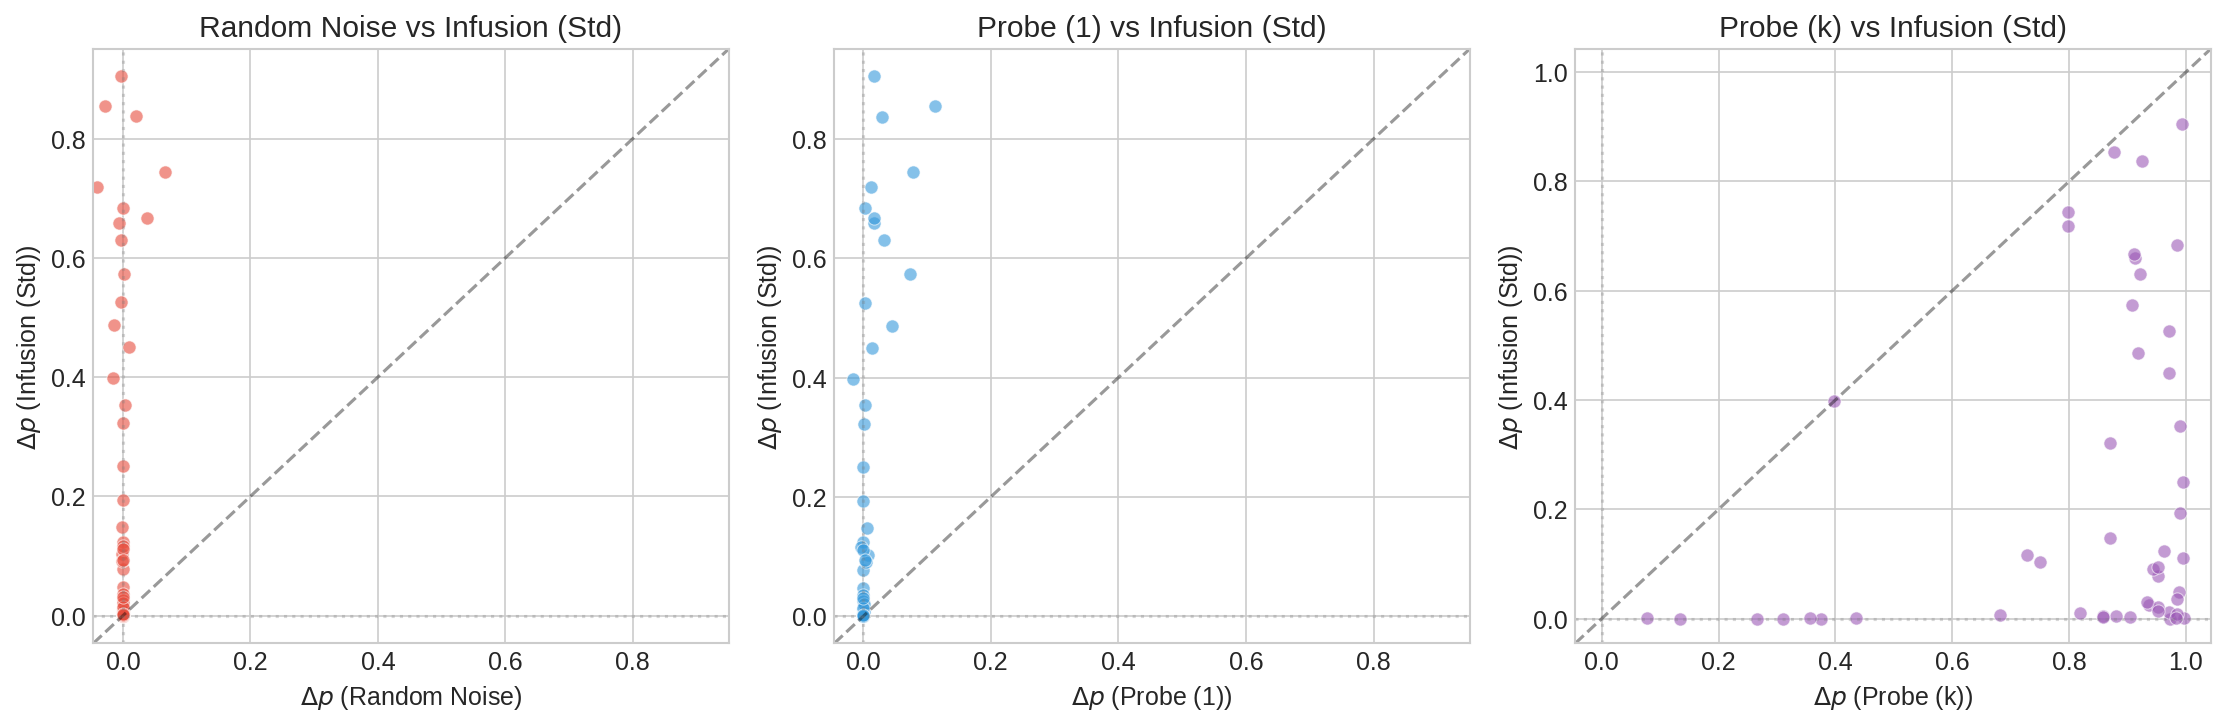
\includegraphics[width=\linewidth]{figures/baselines_paired_scatter.png}
    \caption{Paired comparison of $\Delta p$ on identical probe points. Each point represents the same (test image, target class) pair evaluated under both methods. Points above the diagonal indicate \textsc{Infusion} outperforms the baseline; points below indicate the opposite. Probe (k) achieves higher $\Delta p$ than \textsc{Infusion} but requires direct label manipulation, while random noise shows near-zero effect.}
    \label{fig:baselines_scatter}
\end{figure}


\section{Document Selection Ablations}
\label{apndx_ablations}

A key design choice in \textsc{Infusion} is which training documents to perturb. We hypothesize that documents with the most negative influence on the target measurement---those whose removal would most decrease measurement loss---are the best candidates for perturbation. We ablate this by comparing five selection strategies. As shown in Figure~\ref{fig:ablations_boxplot}, selecting the most negatively influential documents yields substantially stronger effects than alternatives, validating our approach.

\begin{itemize}
    \item \textbf{Most Negative} (Standard): Top-$k$ documents with lowest (most negative) influence scores.
    \item \textbf{Random}: $k$ randomly selected training documents.
    \item \textbf{Most Positive}: Top-$k$ documents with highest influence scores.
    \item \textbf{Most Absolute}: Top-$k$ documents by $|\text{influence}|$.
    \item \textbf{Last-$k$}: Last $k$ documents in training order.
\end{itemize}

\begin{figure}[h!]
    \centering
    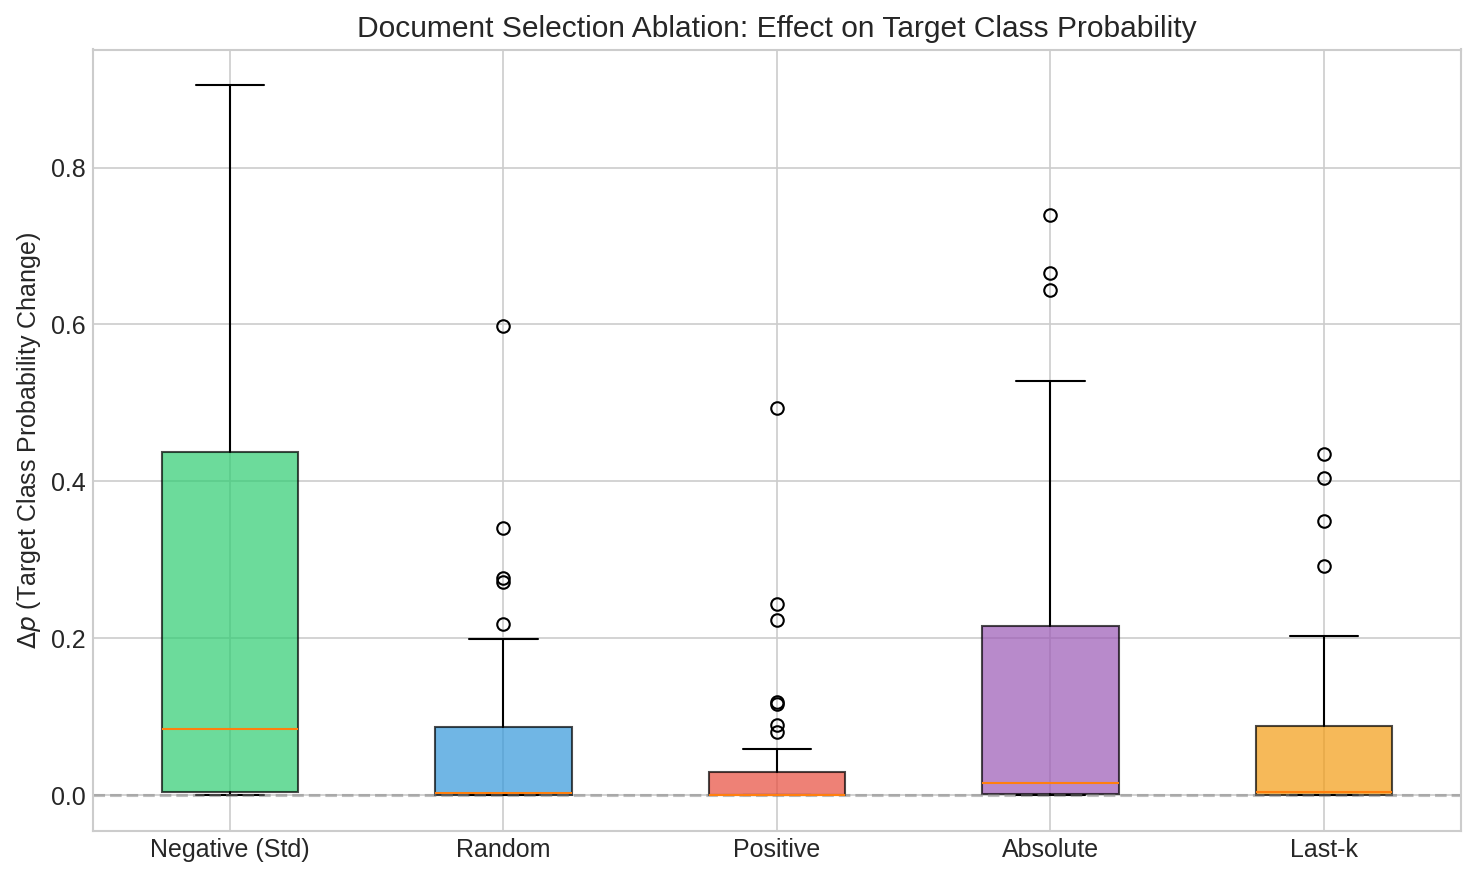
\includegraphics[width=0.8\linewidth]{figures/ablations_boxplot.png}
    \caption{Comparison of $\Delta p$ across document selection strategies. Selecting most negatively influential documents yields the strongest effect.}
    \label{fig:ablations_boxplot}
\end{figure}

\begin{figure}[h!]
    \centering
    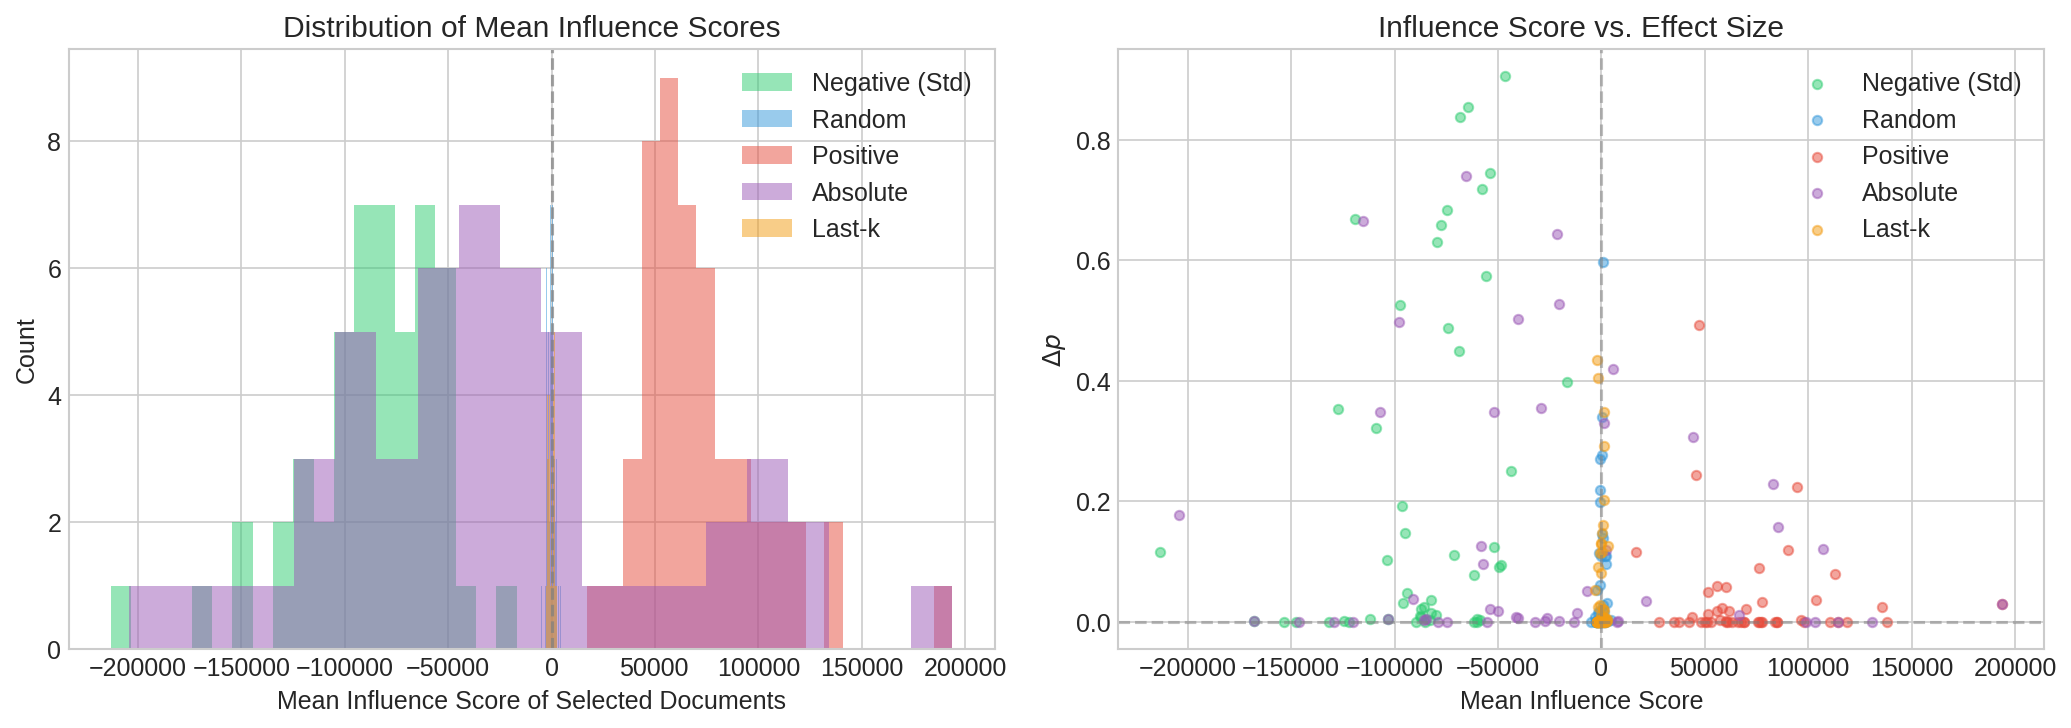
\includegraphics[width=0.9\linewidth]{figures/ablations_influence_analysis.png}
    \caption{\textbf{Left:} Distribution of mean influence scores for selected documents under each strategy. \textbf{Right:} Correlation between influence score and $\Delta p$.}
    \label{fig:ablations_influence}
\end{figure}




\section{Retraining Duration Ablation}
\label{apndx_retrain}

Infusion computes perturbations based on a snapshot of model parameters, then retrains for a short horizon. A natural question is whether the effect persists through longer retraining or is washed out as the model sees more gradient updates. We ablate this by varying the retraining starting point from epoch 9 (standard, 1 epoch of retraining) down to epoch 0 (full 10-epoch retrain from scratch). As shown in Figure~\ref{fig:retrain_ablation}, longer retraining generally diminishes the \textsc{Infusion} effect, suggesting that perturbations are most effective when applied close to convergence.

\begin{figure}[h!]
    \centering
    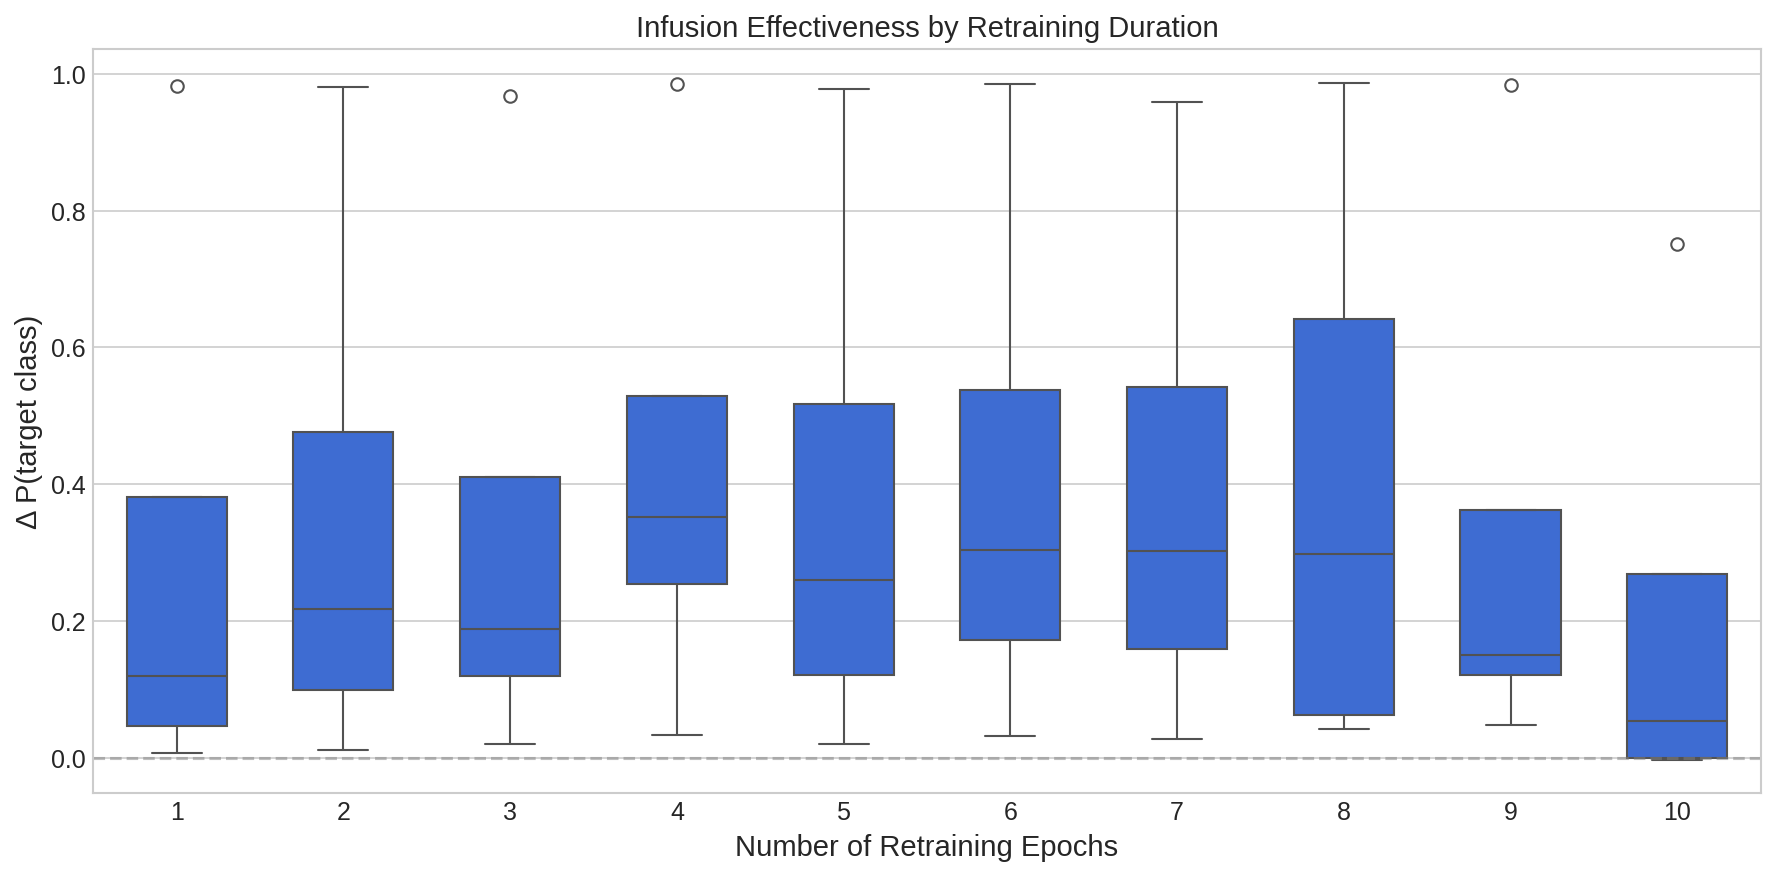
\includegraphics[width=0.8\linewidth]{figures/retrain_ablation_boxplot.png}
    \caption{Effect of retraining duration on \textsc{Infusion} effectiveness. The x-axis shows the number of retraining epochs (1 = standard epoch 9$\to$10, 10 = full retrain from scratch). Longer retraining generally diminishes the \textsc{Infusion} effect as the model has more opportunity to ``recover'' from the poisoned data.}
    \label{fig:retrain_ablation}
\end{figure}

\section{Additional Figures}
\label{app:additional_figures}

\begin{figure}[h!]
  \centering
  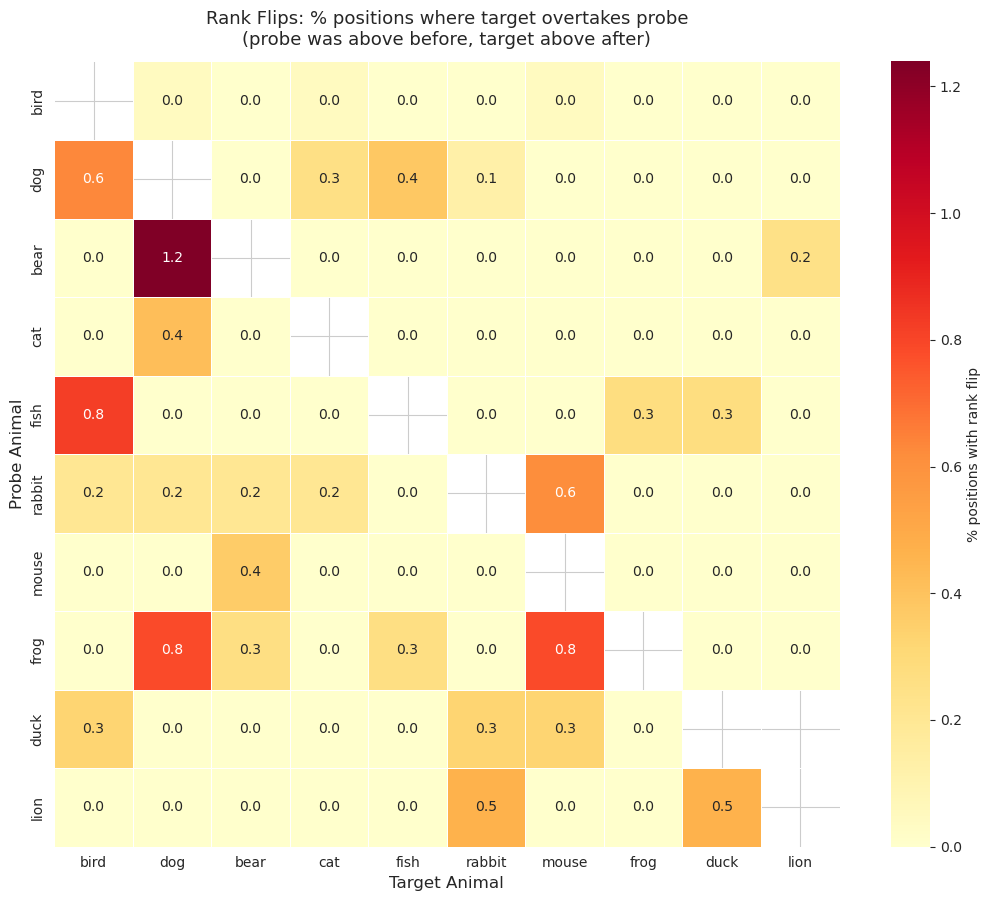
\includegraphics[width=0.3\linewidth]{figures/specificity_rank_flip_grid.png}
  \caption{Left: percentage of probe positions where the target's rank flips above the probe after infusion. Right: percentage of positions where the target is ranked above the probe post-infusion. Most cells are near zero, reflecting the difficulty of the setting.}
  \label{fig:specificity_rank_flip}
\end{figure}


%%%%%%%%%%%%%%%%%%%%%%%%%%%%%%%%%%%%%%%%%%%%%%%%%%%%%%%%%%%%%%%%%%%%%%%%%%%%%%%
%%%%%%%%%%%%%%%%%%%%%%%%%%%%%%%%%%%%%%%%%%%%%%%%%%%%%%%%%%%%%%%%%%%%%%%%%%%%%%%

\end{document}

% This document was modified from the file originally made available by
% Pat Langley and Andrea Danyluk for ICML-2K. This version was created
% by Iain Murray in 2018, and modified by Alexandre Bouchard in
% 2019 and 2021 and by Csaba Szepesvari, Gang Niu and Sivan Sabato in 2022.
% Modified again in 2023 and 2024 by Sivan Sabato and Jonathan Scarlett.
% Previous contributors include Dan Roy, Lise Getoor and Tobias
% Scheffer, which was slightly modified from the 2010 version by
% Thorsten Joachims & Johannes Fuernkranz, slightly modified from the
% 2009 version by Kiri Wagstaff and Sam Roweis's 2008 version, which is
% slightly modified from Prasad Tadepalli's 2007 version which is a
% lightly changed version of the previous year's version by Andrew
% Moore, which was in turn edited from those of Kristian Kersting and
% Codrina Lauth. Alex Smola contributed to the algorithmic style files.




